\chapter[Relation between domain-specific severity profiles and IgG antibody responses in \cfs]{Relation between domain-specific severity profiles and IgG antibody responses in \cfs}
\label{chapter:2024-sym-domains}
\chaptermark{Relation between domain-specific\\severity profiles and IgG antibody responses in \cfs}

%%%%%%%%%%%%%%%%%%%%%%%%%%%%%%%%%%%%%%%%%%%%%%%%%%%%%%%%%%%%%%%%%%%%%%%%
\noindent\underline{J. Malato}, L. Graça, J.-S. Lee, J.M. Cliff, L. Nacul, E.M. Lacerda, and N. Sepúlveda. Relation between domain-specific severity profiles and IgG antibody responses in \cfs. \textit{In preparation}. 2024.

%%%%%%%%%%%%%%%%%%%%%%%%%%%%%%%%%%%%%%%%%%%%%%%%%%%%%%%%%%%%%%%%%%%%%%%%
% \begin{abstract}
% zzz
% \keywords{zzz;zzz}
% \end{abstract}

%%%%%%%%%%%%%%%%%%%%%%%%%%%%%%%%%%%%%%%%%%%%%%%%%%%%%%%%%%%%%%%%%%%%%%%%
%%%%%%%%%%%%%%%%%%%%%%%%%%%%%%%%%%%%%%%%%%%%%%%%%%%%%%%%%%%%%%%%%%%%%%%%
%%%%%%%%%%%%%%%%%%%%%%%%%%%%%%%%%%%%%%%%%%%%%%%%%%%%%%%%%%%%%%%%%%%%%%%%
\section{Introduction}

% context
Myalgic encephalomyelitis/Chronic fatigue syndrome (\cfs) is a disease with unknown aetiology and pathogenesis.
Patients afflicted with this disease experience post-exertional malaise (PEM) after what would be considered normal levels of activity \citep{carruthers2003MyalgicEncephalomyelitis} and long-lasting unexplained fatigue that is not alleviated by rest \citep{fukuda1994ChronicFatigue}, together with a wide range of incapacitating symptoms from various domains, reflecting the effect of specific systems and pathophysiological mechanisms in the body (see Table~\ref{tab:intro-symptom-domains}).
The lack of established biomarkers leaves \cfs diagnosis to be made on the clinical assessment of symptoms and the exclusion of other known diseases that could justify the state of fatigue.
This has led to multiple case definitions for the disease to be proposed over the years \citep{brurberg2014CaseDefinitions, lim2020ReviewCase}, which in practice means that an individual suspected for \cfs could be diagnosed by one criterion and excluded by another \citep{malato2021Statisticalchallenges}.
This lack of diagnostic agreement results in research studies that can present discrepant or even competing results \citep{nacul2019HowHave}.
% resulting in a heterogeneous group of patients .
% Alongside these two, affected individuals experience a wide range of incapacitating symptoms from various domains that also vary in severity, resulting in a symptomatologically diverse group of patients.
% The disease has an estimated prevalence of 0.89\% \citep{lim2020SystematicReviewa}
% , reducing the consistency and reproducibility of finding and 

Additionally, the natural symptom heterogeneity observed across \cfs individuals suggests that ME/CFS is likely an umbrella term, encompassing a spectrum of phenotypically similar illnesses that are included together \citep{malato2023ImpactMisdiagnosis}.
% also contribute to the lack of reproducibility in research.
% In this regard, it is likely that ME/CFS could serve as an umbrella term, encompassing a spectrum of phenotypically similar illnesses that are included together \citep{malato2023ImpactMisdiagnosis}.
% , further hinder the consistency to potential factors for the disease identification of similar cohorts of diagnosed patients \citep{jason2005ChronicFatigue, malato2023ImpactMisdiagnosis}.
As such, dealing with the patients as a whole may be one of the reasons leading to a lack of consistent and reproducible results, possibly due to misdiagnosis of patients.
% there is the proposal of searching for indicators that can help to identify more homogeneous subgroups within this heterogeneous population.
To tackle this, the stratification of suspected cases into similar subgroups could help to identify more specific cluster profiles for research or treatment purposes \citep{jason2005ChronicFatigue, scheibenbogen2017EuropeanME}.
Corroborating this strategy, research studies have shown results on specific subsets of the disease when splitting diagnosed individuals by disease severity or cause of disease onset.
% Consequently, studies have shown results on specific subsets of patients such as disease severity or disease onset.
%, demonstrating that %, indicating that the implementation of stratification methods could \red{bear good results}.
For instance, \citet{montoyaCytokineSignatureAssociated2017} correlated proinflammatory cytokines with disease severity in patients, and \citet{cliff2019CellularImmune} split \cfs into subgroups for mild--moderate and severely affected individuals and found increased mucosal-associated invariant T (MAIT) lymphocytes in the latter subgroup, suggesting the effect of the immune system in the exacerbation of the observed symptoms.
Other studies have demonstrated differences in subsets reporting acute response to a herpesviruses infection prior to the development of the disease \citep{domingues2021HerpesvirusesSerologya, sepulveda2022RevisitingIgG, domingues2023AssociationAnalysis}.
These results are in line with the hypothesis that at least a subset of \cfs patients has an autoimmune aetiology, which could characterise the significant portion of cases reporting a previous infection-like event before the development of the disease \citep{sotznyMyalgicEncephalomyelitisChronic2018}.
% and an increasing number of results supporting the the role of an infection as a trigger for \cfs in the autoimmune hypothesis \citep{sotznyMyalgicEncephalomyelitisChronic2018}.
However, there is still no unified strategy to subtype \cfs \citep{jason2005ChronicFatigue}.
% despite multiple pathological proposals, there is still no unified strategy to further subgroup ME/CFS individuals \citep{jason2005ChronicFatigue}.


\bsni
% ----------------------------------------------------------------------
% Objective
The aim of this preliminary study is to increase our understanding of how related symptoms could explain the response towards six different herpesviruses.
% MDS
We first studied the symptomatic heterogeneity across \cfs patients and healthy controls to look for possible discernible clusters.
% LCA
Then, we categorised the symptoms by seven domains (immunological, neuroendocrine, PEM, autonomic, neurocognitive, neurophysiological, and pain) and identified subgroups based on similar profiles of severity.
As such, instead of analysing the relationship between all symptoms screened at diagnosis, we considered the seven domains as specific phenotypes associated with particular mechanisms and stratified them instead.
% by their increasing degree of severity.
Afterwards, antibody IgG concentrations and population seroprevalence towards distinct herpesviruses were measured across the domain subgroups and compared with healthy controls.

The results here presented are part of an undergoing study.
Future work will look to study the combinations of domain severity from each individual to ascertain more complete patterns of classification of the disease.


% analysed the possible stratification of \cfs patients through the creation of multiple severity subgroups based on the combination of specific symptoms related to domains usually assessed in diagnosis.
% Using data from the UK ME/CFS Biobank (UKMEB) we studied the symptomatic heterogeneity across \cfs patients and healthy controls to look for possible discernible clusters.
% Then, we split the symptoms into seven domains (immunological, neuroendocrine, PEM, autonomic, neurocognitive, neurophysiological, and pain) and identified subgroups based on profiles of severity similarity.
% As such, instead of analysing the relationship between all symptoms screened at diagnosis, we grouped mechanistically similar symptoms and stratified \cfs individuals by their combined severity.

% We tried to go beyond the binary strategies of symptom classification (absent vs. present, mild vs. severe), by looking at the symptoms that implementing 

% strategy of classifying individuals based on two binary absence--presence 

% We used data from symptoms from the UK ME/CFS Biobank (UKMEB) to 
% \citep{lacerda2017UKME, lacerda2018UKME}

% Usual case criteria \citep{carruthers2003MyalgicEncephalomyelitis} and the UK ME/CFS Biobank (UKMEB) have proposed distinct domains
% - Advantages of having a more granular distinction of distinct phenotypic groups of ME/CFS patients to study different mechanisms of dysregulation, in the case of autoimmunity [cite], exacerbated responses to external pathogens or chronic latent reinfections [cite], etc.
% - Definition/Justification of each domain

% . UKMEB description \citep{lacerda2017UKME, lacerda2018UKME}



% For the diagnosis of \cfs, the presence and severity of multiple symptoms are assessed.
% These symptoms are usually viewed as part of distinct domains, reflecting the effect of specific systems and pathophysiological mechanisms in the body (Table~\ref{tab:intro-symptom-domains} in Chapter~\ref{chapter:introduction}).
% Depending on the case definition used, the presence and absence of a number of symptoms


% Symptoms assessed during the diagnosis for ME/CFS are usually included into distinct domains relating the effect of specific systems and pathophysiological mechanisms in the body (Table~\ref{tab:intro-symptom-domains} in Chapter~\ref{chapter:introduction}).
% Its assessment 
% These

% Usual case criteria \citep{carruthers2003MyalgicEncephalomyelitis} and the UK ME/CFS Biobank (UKMEB) have proposed distinct domains

% hen it comes to the symptoms assessed in ME/CFS, the 
% Specific symptoms

% One proposal, is to aggregate patients by severity of symptoms.
% For instance, 


% - Other ideas for stratification that could provide insights into the disease
%     - Jason 2005
    

% - Limitations to go further due to patients heterogeneity and symptom heterogeneity
% Criterion variability is the largest source of uncertainty

% - Proposal of stratification and creation of subgroups based on combination of specific symptoms related to particular domains
% - Advantages of having a more granular distinction of distinct phenotypic groups of ME/CFS patients to study different mechanisms of dysregulation, in the case of autoimmunity [cite], exacerbated responses to external pathogens or chronic latent reinfections [cite], etc.
% - Definition/Justification of each domain
% Domain definitions:
% \note{Autonomic nervous system}: Autonomic-related dysfunctions that could generate symptoms in line with autonomic imbalance or orthostatic hypertension (nausea, dizziness while- or intolerance to standing up, lightheadedness, or palpitations), heart rate and blood pressure/impaired circulation (pallor), autonomic reflexes, etc.
% \note{Immunological}
% \note{Neurological cognitive (neurocognitive)}
% \note{Neuroendocrine}
% \note{Neurophysiological}
% \note{Pain}
% \note{PEM}
% and periods of impaired circulation compatible with autonomic dysfunction


%%%%%%%%%%%%%%%%%%%%%%%%%%%%%%%%%%%%%%%%%%%%%%%%%%%%%%%%%%%%%%%%%%%%%%%%
%%%%%%%%%%%%%%%%%%%%%%%%%%%%%%%%%%%%%%%%%%%%%%%%%%%%%%%%%%%%%%%%%%%%%%%%
%%%%%%%%%%%%%%%%%%%%%%%%%%%%%%%%%%%%%%%%%%%%%%%%%%%%%%%%%%%%%%%%%%%%%%%%
\section{Materials and methods}


%%%%%%%%%%%%%%%%%%%%%%%%%%%%%%%%%%%%%%%%%%%%%%%%%%%%%%%%%%%%%%%%%%%%%%%%
%%%%%%%%%%%%%%%%%%%%%%%%%%%%%%%%%%%%%%%%%%%%%%%%%%%%%%%%%%%%%%%%%%%%%%%%
\subsection{Study participants}

Throughout the initial stages of the study, we worked with a total sample size of 347 individuals split into two cohorts of 241 ME/CFS patients and 106 healthy controls matched for sex and age.
All participants were adults and part of the UK ME/CFS Biobank (UKMEB) \citep{lacerda2017UKME}.
ME/CFS patients were ascertained for compliance by the 1994 US Centre for Disease Control and Prevention Criteria (CDC-1994, \citealt{fukuda1994ChronicFatigue}) or the 2003 Canadian Consensus Criteria (CCC-2003, \citealt{carruthers2003MyalgicEncephalomyelitis}).
According to the biobank, aside from the diagnosis requirements, patients would be excluded if they (i) used drugs known to alter immune function in the preceding three months or antiviral medication; (ii) had any vaccinations in the preceding three months; (iii) had a history of acute and chronic infectious diseases (but not herpes viruses); (iv) were diagnosed with another severe illness such as cancer, coronary heart disease, or uncontrolled diabetes; (v) had a severe mood disorder; (vi) had been pregnant or breastfeeding in the preceding 12 months; or (vii) were morbidly obese (BMI ${\geq 40}$ kg/m${^2}$).
Additional information related to the recruitment and inclusion of individuals and management of samples by the UKMEB can be found elsewhere \citep{lacerda2017UKME, lacerda2018UKME}.

Similar to previous studies (\citealt{cliff2019CellularImmune, domingues2023AssociationAnalysis}; Chapter~\ref{chapter:2023-sym-and-herpesvirus}), age, sex, and disease duration were summarised and compared across healthy controls and patients (Supplementary Table~\ref{appendix:taba1-population-description}).
Pearson's $\chi^2$ test was applied to qualitative measures, and the non-parametric two-sided Kruskal-Wallis rank sum test was applied to quantitative values.
All statistical tests were performed using a significance level of 5\%.

% Supplementary Table 1
% Supplementary Table~\ref{appendix:taba1-population-description}


%%%%%%%%%%%%%%%%%%%%%%%%%%%%%%%%%%%%%%%%%%%%%%%%%%%%%%%%%%%%%%%%%%%%%%%%
%%%%%%%%%%%%%%%%%%%%%%%%%%%%%%%%%%%%%%%%%%%%%%%%%%%%%%%%%%%%%%%%%%%%%%%%
\subsection{Symptomatology assessment}

At enrolment, all participants were asked to answer a symptom assessment form related to the severity range of 57 specific symptoms experienced over the previous seven days (Supplementary Table~\ref{appendix:taba2-sym-description}).
Each symptom was rated within an ordinal scale with four possible degrees of severity: absent, mild, moderate, or severe.
This symptom assessment was included as part of a questionnaire for ME/CFS diagnosis.
% We made use of the answers given by the ME/CFS patients only.

% Supplementary Table 2
% Supplementary Table~\ref{appendix:taba2-sym-description}

During data preprocessing, the relative frequency of each symptom in the ME/CFS study population was calculated (Figure~\ref{fig:figa1-ordinal-symptom-proportion-by-absent}).
Symptoms with a frequency of unreported answers higher than 20\% were identified and removed.
Ultimately, 10 symptoms surpassed the missing data threshold and were removed from the study, leaving the analyses to be performed with the remaining 47.
The symptoms removed were intolerance to alcohol (alcoholintoler), pain in chest and/or abdomen (chestabdpain), unusually cold hands and/or feet (coldhandsfeet), difficulty retaining information (diffdecisions), difficulty finding or saying words (diffwords), fatigue or exhaustion lasting for more than 24 hours after what would be considered normal levels of activity (fatiguelast24h), palpitations and irregular heartbeats (palpitations), feeling sick or nauseated (sick\_nausea), muscle twitching (twitching), and abnormal appetite and/or significant changes in weight (weightchange).

\begin{figure}[htbp]
    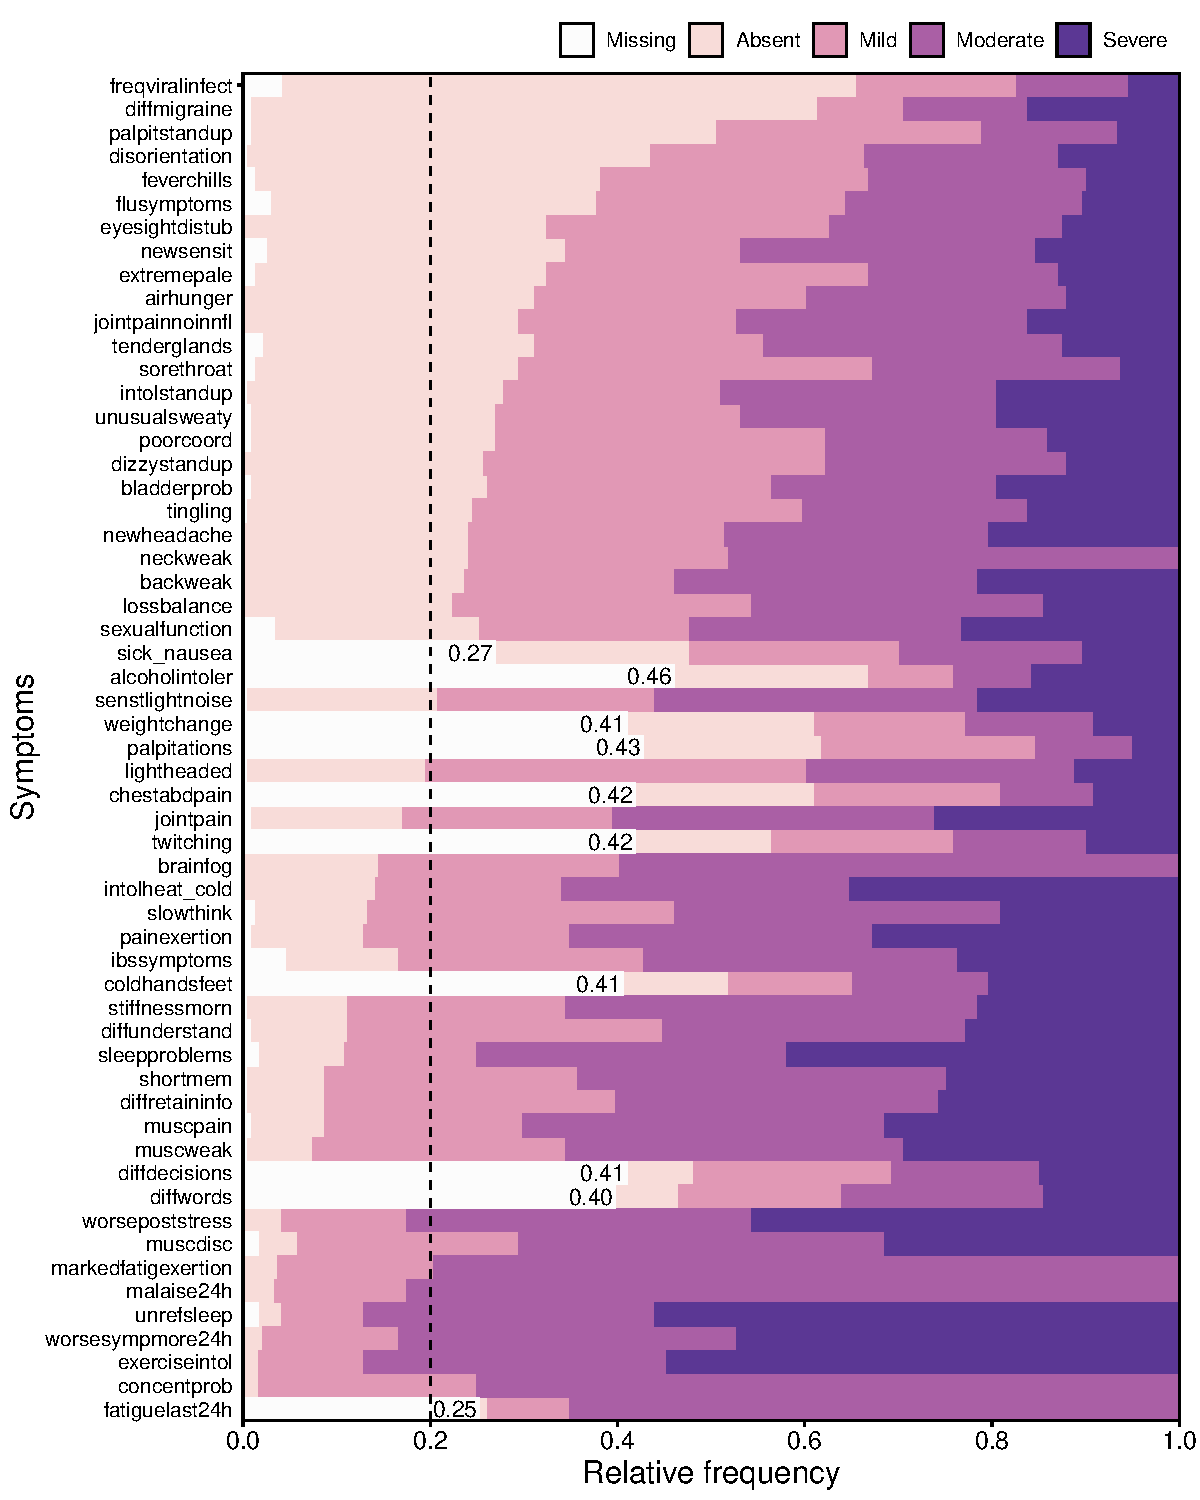
\includegraphics[width=0.95\textwidth]{chapter/2024-sym-domains/figures/figa1-ordinal-symptom-proportion-by-absent.pdf}
    \caption[Relative frequency of ordinal degrees of severity on each one of the original 57 symptoms available across the population of ME/CFS patients]{Relative frequency of ordinal degrees of severity on each one of the original 57 symptoms available across the population of ME/CFS patients ($n = 241$). Symptoms are ordered by decreasing level of severity and relative proportion. Vertical dashed line at the 0.2 mark designates the missing values cutoff. Symptoms with a proportion of unreported (missing) severity across all individuals higher than that value were identified (relative proportions that surpass the cutoff are indicated in the missing columns) and removed from the analysis. A more detailed description of each symptom can be found elsewhere (Supplementary Table~\ref{appendix:taba2-sym-description}).}
    \label{fig:figa1-ordinal-symptom-proportion-by-absent}
\end{figure}
% Figure 1
% Figure~\ref{fig:figa1-ordinal-symptom-proportion-by-absent}

% Supplementary Figure 1
% Supplementary Figure~\ref{fig:figa1-ordinal-symptom-proportion-by-absent}

%%%%%%%%%%%%%%%%%%%%%%%%%%%%%%%%%%%%%%%%%%%%%%%%%%%%%%%%%%%%%%%%%%%%%%%%
%%%%%%%%%%%%%%%%%%%%%%%%%%%%%%%%%%%%%%%%%%%%%%%%%%%%%%%%%%%%%%%%%%%%%%%%
\subsection{Herpesviruses serological data}

Plasma samples from eligible patients were collected for quantification of immunoglobulin G (IgG) antibodies against human cytomegalovirus (CMV), Epstein-Barr virus (EBV) nuclear antigen-1 (EBV EBNA1) and EBV viral capsid antigen (EBV VCA), human herpesvirus-6 (HHV6), herpes simplex virus 1 (HSV-1), herpes simplex virus 2 (HSV-2), and varicella-zoster virus (VZV).
Concentration assays were measured by commercial quantitative ELISA and expressed in arbitrary units per millilitre (U/ml).
Seropositivity cutoff of each herpesvirus was determined according to the manufacturer's instructions.
Under those assumptions, individuals were classified as seronegative or seropositive, with some individuals being considered equivocal.
In this study, we treated equivocal individuals as seronegative.
More information related to the laboratory procedures can be found in previous studies \citep{cliff2019CellularImmune, domingues2021HerpesvirusesSerologya}.

The use of both data on antibody titrations and seroprevalence serves to complement inferences when comparing cohorts.
Since antibodies against different herpesviruses can vary, the analysis of seroprevalence is useful in a context where IgG concentrations tend to be lower, with the population more homogeneously split between seronegative and seropositive.


%%%%%%%%%%%%%%%%%%%%%%%%%%%%%%%%%%%%%%%%%%%%%%%%%%%%%%%%%%%%%%%%%%%%%%%%
%%%%%%%%%%%%%%%%%%%%%%%%%%%%%%%%%%%%%%%%%%%%%%%%%%%%%%%%%%%%%%%%%%%%%%%%
\subsection{Symptoms intra- and inter-rater agreement}

We used the 47 selected symptoms, each characterised by four possible degrees of severity, to quantify the similarity of symptoms for each one of the healthy controls and ME/CFS-diagnosed individuals in the data set (intra-rater agreement).
We computed the overall severity proportions and estimated the entropy using the usual (Shannon) formula \citep{shannon1948MathematicalTheory},
% 
$$H(X) = - \sum_{k = 1}^{4} p_{ik} \log_2 p_{ik} \ ,$$% i = 1, \ldots, n \ ,$$
% 
where, for an individual $i$, $p_{ik}$ represents the proportion of each one of the severity levels $k$ (in the equation, $k = \{1, 2, 3, 4\}$ represents the four categories of severity, with values 1 for absent, 2 for mild, 3 for moderate, and 4 for severe).
On each individual, this proportion for a severity category $k$ varies between 0 (non-existent across symptoms) and 1 (all symptoms with the same degree of severity), and the total sum of all four proportions equals 1.
As a result, in cases where an individual experiences the exact same severity level across all symptoms, the estimated entropy would be 0.
%, the highest possible homogeneity.
Conversely, in a scenario where a patient demonstrates an extremely heterogeneous profile, with a high degree of fluctuation from one symptom to the other, we can assume that the severity level follows a Uniform distribution on each symptom with the resulting proportions for the four levels being equally split at 25\% ($\frac{1}{4} = 0.25$).
Under this scenario, the estimated entropy would reach its maximum possible value of 2 (maximum value of entropy estimated as $\log_2 k$; in this case, we have $\log_2 4 = 2$), signifying maximal uncertainty or diversity in the symptomatological severity pattern of an individual.

To compare the similarity between the severity profile of all 347 participants (inter-rater agreement), we iteratively calculated a pairwise similarity matrix between each two individuals by estimating the Cohen's $\kappa$ coefficient \citep{cohen1960CoefficientAgreement}.
Afterwards, the resulting similarity matrix was analysed by classical multidimensional scaling (MDS).
%, which, similarly to a principal component analysis, can be used to identify groups of similar individuals with regard to their symptom severity profile.
More information on this method can be seen in a previous application to similar data from the UKMEB \citep{malato2021Statisticalchallenges}.


%%%%%%%%%%%%%%%%%%%%%%%%%%%%%%%%%%%%%%%%%%%%%%%%%%%%%%%%%%%%%%%%%%%%%%%%
%%%%%%%%%%%%%%%%%%%%%%%%%%%%%%%%%%%%%%%%%%%%%%%%%%%%%%%%%%%%%%%%%%%%%%%%
\subsection{Construction of patient subgroups from symptomatological data}

Originally, the symptoms recorded were grouped into seven distinct domains: autonomic ($n = 8$), immunological ($n = 7$), neurological cognitive (neurocognitive) ($n = 16$), neuroendocrine ($n = 4$), pain ($n = 5$), post-exertional malaise (PEM, $n = 5$), and sleep function ($n = 2$).
This grouping scheme arises from the detailed description of symptoms in the CCC-2003 criteria and from conversations with specialised clinicians at the UKMEB.
It serves as a way to organise the potentially afflicted systems and trace back from the combination of expressed symptoms.
For this study, the two symptoms related to sleep dysfunction (sleepproblems and unrefsleep) were included in the neurophysiological domain ($n = 7$), which is a larger group that also included other symptoms from both autonomic and neurocognitive domains (Supplementary Table~\ref{appendix:taba2-sym-description}).
Henceforth, analysis and stratification of ME/CFS patients were done considering the entirety of symptoms and considering symptoms split into the seven domains.

We implemented the latent class analysis (LCA) modelling method on the severity profiles of ME/CFS patients.
Considering all symptoms or each domain, this probabilistic algorithm identifies subgroups (or latent classes) in the symptoms' multivariate categorical data that have a similar profile of severity.
Simply put, it defines ``clusters'' of similar patients, estimating the posterior probability that relates each individual to each one of the proposed subgroups.

Since the number of latent classes in the model is a predetermined parameter required before performing the LCA, we tested different models by sequentially increasing the parameter value between 2 and 10.
This means that, at the bare minimum, we performed LCA considering the ME/CFS population to be stratified into two subgroups; and at the maximum, and admitting a highly heterogeneous symptomatological profile from the patients, the model clustered the patients into ten groups.

The optimal number of latent classes in the models was initially chosen based on the Akaike and the Bayesian information criteria (AIC and BIC, respectively).
Both information criteria evaluate and reward goodness of fit while at the same time penalising for the number of parameters considered.
This is a way to adjust for the model's complexity and avoid overfitting, with the goal being to choose a more parsimonious model.
Looking at the formulas for AIC ($\text{AIC} = -2\ln(\hat{L}) + 2k$), and BIC ($\text{BIC} = -2\ln(\hat{L}) + k\ln(n)$), respectively, $\ln(\hat{L})$ is the maximised log-likelihood function for the model, $k$ is the number of parameters, and $n$ is the sample size used.
Therefore, under the principle of parsimony, for a set of candidate models, the ``best'' model will be the one presenting the smallest score value for AIC or BIC.
Because the penalty term varies between the two information criteria, it is likely that the selected models for the same domain have a different number of classes.
AIC adds a direct penalty related to the number of parameters in the model (term $2k$).
BIC penalty increases logarithmically with sample size (term $k\ln(n)$).
This makes BIC the more strict criteria of the two and one should expect it to go for models with fewer parameters.

Once the model with optimal number of latent groups was chosen in each domain, the estimated subgroups were ordered based on the increasing symptom severity profile according to the LCA class membership probabilities.
For the subgroups of each domain, a sequential number was attributed, meaning that any group denominated `g1' classifies individuals within a pattern of reduced severity (mostly absent to mild).
Oppositely, subgroups of higher numbers classify the population with a more severe combination of symptoms.


%%%%%%%%%%%%%%%%%%%%%%%%%%%%%%%%%%%%%%%%%%%%%%%%%%%%%%%%%%%%%%%%%%%%%%%%
%%%%%%%%%%%%%%%%%%%%%%%%%%%%%%%%%%%%%%%%%%%%%%%%%%%%%%%%%%%%%%%%%%%%%%%%
\subsection{Analysis of serological data}

With ME/CFS patients stratified by multiple subgroups,
% depending on the symptomatological domains, 
we compared both antibody concentration and seropositivity values against healthy controls with the intent of identifying differences that would relate the profile of symptom severity 
% from one or more domains 
and past exposure to the assessed herpesviruses.
For each virus, we performed two complementary analyses.
First, a two-sided Kruskal-Wallis sum rank test was used to compare the median IgG antibody concentration values (${\log_{10}}$-transformed) on healthy controls and ME/CFS subgroups.
We then proceeded with the test's extension, the non-parametric pairwise Mann-Whitney U test, to perform comparisons within population pairs.
Second, we created contingency tables for the number of seropositive and seronegative individuals across the cohorts for healthy controls, ME/CFS patients as a whole, and each one of the domains' subgroups, and tested whether there were differences in population frequencies.
We used Pearson's $\chi^2$ for independence on comparisons across multiple cohorts, followed by a pairwise Fisher's exact test to iteratively compare between two groups.
On both analyses, the level of significance was set at 5\%.
All estimated (raw) p-values were adjusted for multiple testing post-hoc, using the Benjamini-Hochberg procedure \citep{benjaminiControllingFalseDiscovery1995}, ensuring a global false discovery rate of 5\%.


%%%%%%%%%%%%%%%%%%%%%%%%%%%%%%%%%%%%%%%%%%%%%%%%%%%%%%%%%%%%%%%%%%%%%%%%
%%%%%%%%%%%%%%%%%%%%%%%%%%%%%%%%%%%%%%%%%%%%%%%%%%%%%%%%%%%%%%%%%%%%%%%%
\subsection{Statistical software}

All statistical analyses were conducted using the R software, version 4.2.3 (2023-03-15) \citep{rcoreteamLanguageEnvironmentStatistical2020}.
For the LCA on polytomous outcomes variables we used the package \textit{poLCA} \citep{linzer2011PoLCAPackage} 
% , which uses both expectation-maximisation and Newton-Raphson algorithms to find the maximum likelihood estimates of each model parameter.
and to estimate inter-rater agreement between pairs of individuals we used the package \textit{irr} \citep{gamer2012irr}.


%%%%%%%%%%%%%%%%%%%%%%%%%%%%%%%%%%%%%%%%%%%%%%%%%%%%%%%%%%%%%%%%%%%%%%%%
%%%%%%%%%%%%%%%%%%%%%%%%%%%%%%%%%%%%%%%%%%%%%%%%%%%%%%%%%%%%%%%%%%%%%%%%
%%%%%%%%%%%%%%%%%%%%%%%%%%%%%%%%%%%%%%%%%%%%%%%%%%%%%%%%%%%%%%%%%%%%%%%%
\section{Results}

%%%%%%%%%%%%%%%%%%%%%%%%%%%%%%%%%%%%%%%%%%%%%%%%%%%%%%%%%%%%%%%%%%%%%%%%
%%%%%%%%%%%%%%%%%%%%%%%%%%%%%%%%%%%%%%%%%%%%%%%%%%%%%%%%%%%%%%%%%%%%%%%%
\subsection{Characterisation of study participants}

A summary of the basic characteristics of the study population and considered subpopulations, based on severity and infection trigger, can be found in Supplementary Table~\ref{appendix:taba1-population-description}.
Both study cohorts of healthy controls and ME/CFS had more female patients than males, almost at a ratio of 3 to 1 (Pearson's $\chi^2$ test, p = 0.819).
The average age was 41.7 and 42.2 years old, respectively, for healthy individuals and patients (Kruskal-Wallis test, p = 0.827).
ME/CFS patients had an average of 12.4 years of disease duration and the large majority was diagnosed by both the CDC-1994 and CCC-2003 ($n = 205$, 85.1\%), with fewer individuals diagnosed by only the former ($n = 33$, 13.7\%), or the latter ($n = 3$, 1.2\%).

The ME/CFS subgroups for mild to moderate ($n = 188$, 78.0\%) and severely affected patients ($n = 53$, 22.0\%) did not differ substantially in sex or age distribution.
However, severe patients had significantly longer duration of the disease by an average of 4.4 years (median difference = 5.9 years, Kruskal-Wallis test, p = 0.001), and had all but one individual diagnosed by both diagnoses (Pearson's $\chi^2$ test, p = 0.004).

The four infection trigger-based subgroups also had similar sex (p = 0.642), disease duration (p = 0.495), and age distributions (p = 0.338).
Mean ages were 43.5, 40.2, 43.1, and 40.5 years old for patients who did not know their disease trigger (S0), patients who reported a non-infection trigger (S1), patients who reported an infection trigger but the infection was not confirmed by a lab test (S2), and patients who reported an infection trigger with that infection confirmed by a lab test (S3), respectively.
Differently from the binary severity subgroups, there were no significant differences in the diagnosis used on the participants of each subgroup (p = 0.095).


%%%%%%%%%%%%%%%%%%%%%%%%%%%%%%%%%%%%%%%%%%%%%%%%%%%%%%%%%%%%%%%%%%%%%%%%
%%%%%%%%%%%%%%%%%%%%%%%%%%%%%%%%%%%%%%%%%%%%%%%%%%%%%%%%%%%%%%%%%%%%%%%%
\subsection{Symptom description and similarity profiles}

% description
In the ME/CFS population, the distribution of severity levels varied among symptoms (Figure~\ref{fig:figa1-ordinal-symptom-proportion-by-absent}).
Certain symptoms, such as frequent viral infections (freqviralinfect, immunological domain) and different or worse migraines (diffmigraine, pain domain), were absent in the majority of patients, marked as such in 61.4\% and 60.6\% of the population, respectively.
Notably, absent values only appeared in an average of 19.6\% of cases across all symptoms.
% (SD = 13.8\%) across all symptoms.
Moderate was the predominant severity level overall, manifesting on average in 31.2\% of cases.
% (SD = 15.8\%).
Conversely, only two symptoms appeared as severe in the majority of patients: unrefreshing sleep (unrefsleep, neurophysiological domain) and intolerance to exercise (exerciseintol, PEM domain and a requisite for the CCC-2003 diagnosis), with 56.0\% and 54.8\% of the patients study population marking them as severe, respectively.

Among the 47 selected symptoms, five did not exhibit the maximum value of severity.
These were neck weakness (neckweak), brain fog (brainfo), and difficulties in concentrating (concentprob), from the neurocognitive domain, and long-lasting marked physical or mental fatigue and malaise after what would be considered minimal/normal levels of exertion (markedfatigexertion and malaise24h), belonging to the PEM domain.
Interestingly, despite not including severe as a severity level, with the exception of brainfog, these symptoms had close to no absent values, being predominantly marked as moderate or mild.

% \subsubsection{Intra-rater agreement}

% entropy
The individual estimated entropy values in the population varied between 0.00 and 1.99, the minimal and almost-maximal possible values, respectively (Figure~\ref{fig:fig1-id-entropy-and-mds}A).
There were clear differences between healthy controls and ME/CFS patients.
Individuals from the healthy population were the only ones with high levels of homogeneity in all symptoms.
Of the 106 healthy participants, 13 (12.26\%) consistently reported the absence of any symptoms, with the large majority ($n = 91$, 85\%) displaying entropy below the midrange value of 1.00.
Conversely, the lowest reached entropy in the ME/CFS population was 0.66, with 235 (97.51\%) patients reporting estimates above the midrange value.
This showed that at the individual level, no \cfs patient experienced the same severity level across all recorded symptoms, which, similarly to some healthy controls, would result in an entropy value of zero.
The more consistent ME/CFS individuals identified most of their symptoms as either moderate with some mild symptoms or severe with some moderate symptoms.
These results indicated that a majority of patients exhibited a heterogeneous combination of severity levels across the assessed symptoms, which contrasted with the cohort of healthy controls that exhibited lower entropy due to the absence of symptoms.

\begin{figure}[htbp]
    \centering
    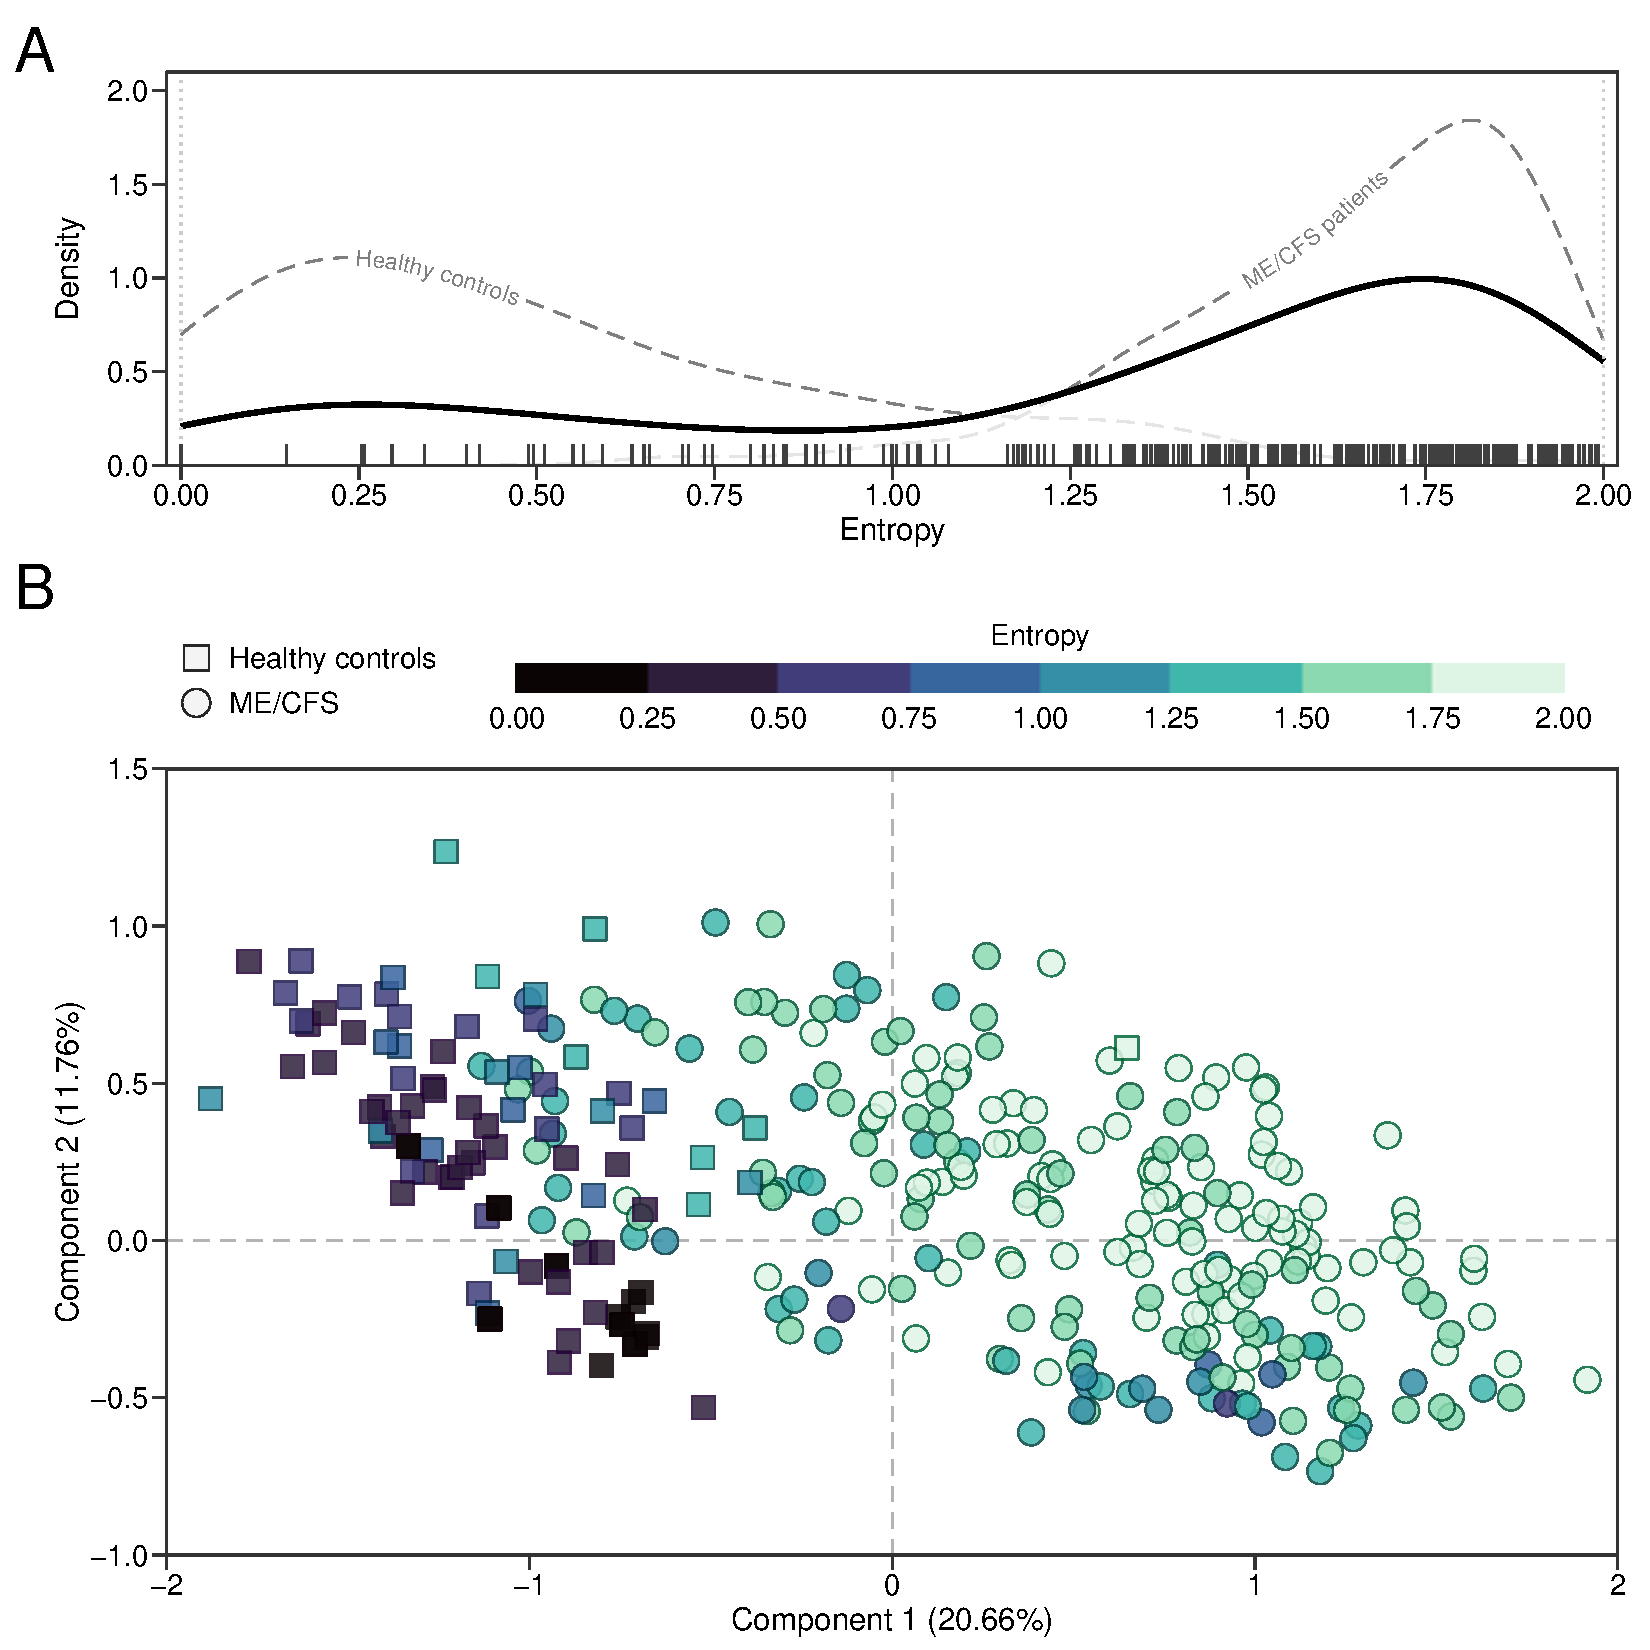
\includegraphics[width=0.9\textwidth]{chapter/2024-sym-domains/figures/fig1-id-entropy-and-mds.pdf}
    \caption[Estimation of intra- and inter-rater agreement to assess heterogeneity on the combination of severity levels across the study population]{Estimation of intra- and inter-rater agreement to assess heterogeneity on the combination of severity levels across the study population. (A) Kernel density estimation of entropy values of the study population (dark line) and individualised cohorts (light-gray dashed lines), with entropy values of each participant identified (rug plot/vertical dashes displayed along the $x$-axis); (B) Classical multidimensional scaling (MDS) based on Cohen's $\kappa$ coefficient, assessing the similarity of symptoms between participants.}
    \label{fig:fig1-id-entropy-and-mds}
\end{figure}
% Figure 2
% Figure~\ref{fig:fig1-id-entropy-and-mds}

% \subsubsection{Inter-rater agreement}

% MDS
Comparing the inter-rater profile similarity, classical MDS results for the first two components explained 32.42\% of the total variance (Figure~\ref{fig:fig1-id-entropy-and-mds}B).
The first component discriminated between healthy controls and ME/CFS patients.
Healthy individuals appeared as the more homogeneous group, with individuals being more closely related than the patients' cohort.
The second component seemed to correlate well with entropy, identifying clusters in both cohorts where estimated entropy was lower.
Interestingly, the cluster of patients sharing lower values of entropy was the farthest away from healthy controls and identified the ME/CFS group of individuals exhibiting elevated levels of severity on a majority of symptoms (i.e., those considered by clinicians to be severely affected).
From the results it is evident that there is a high degree of heterogeneity among the severity profile of assessed symptoms from patients.
Only patients at the two opposite extremes showed reduced estimates for entropy: those with reduced severity levels, closer to healthy controls (but still with higher entropy than healthy controls), and those with severe ME/CFS.
Patients in between displayed high variability in entropy and symptom profile.


%%%%%%%%%%%%%%%%%%%%%%%%%%%%%%%%%%%%%%%%%%%%%%%%%%%%%%%%%%%%%%%%%%%%%%%%
%%%%%%%%%%%%%%%%%%%%%%%%%%%%%%%%%%%%%%%%%%%%%%%%%%%%%%%%%%%%%%%%%%%%%%%%
\subsection{Latent class analysis across symptomatological domains}

% LCA number of criteria for domains (AIC & BIC)
Latent class models were applied considering 47 symptoms combined into seven domains: immunological ($n = 7$), neuroendocrine ($n = 4$), PEM ($n = 5$), autonomic ($n = 8$), neurocognitive ($n = 16$), neurophysiological ($n = 7$), and pain ($n = 5$) (Supplementary Table~\ref{appendix:taba2-sym-description}).
According to AIC, the optimal number of subgroups (or latent classes) when studying the combination of all symptoms was five (domain Total in Figure~\ref{fig:fig2-aic-bic-number-of-classes}A).
When considering different domains at a time, the best LCA models identified 3, 4, 4, 5, 6, 6, and 6, respectively, for the immunological, neuroendocrine, PEM, autonomic, neurocognitive, neurophysiological, and pain domains.
Conversely, BIC selected the minimum possible number of classes for the immunological and neuroendocrine domains, stratifying the rest into three classes, including the stratification done considering all symptoms (Figure~\ref{fig:fig2-aic-bic-number-of-classes}B).

\begin{figure}[h]
    \centering
    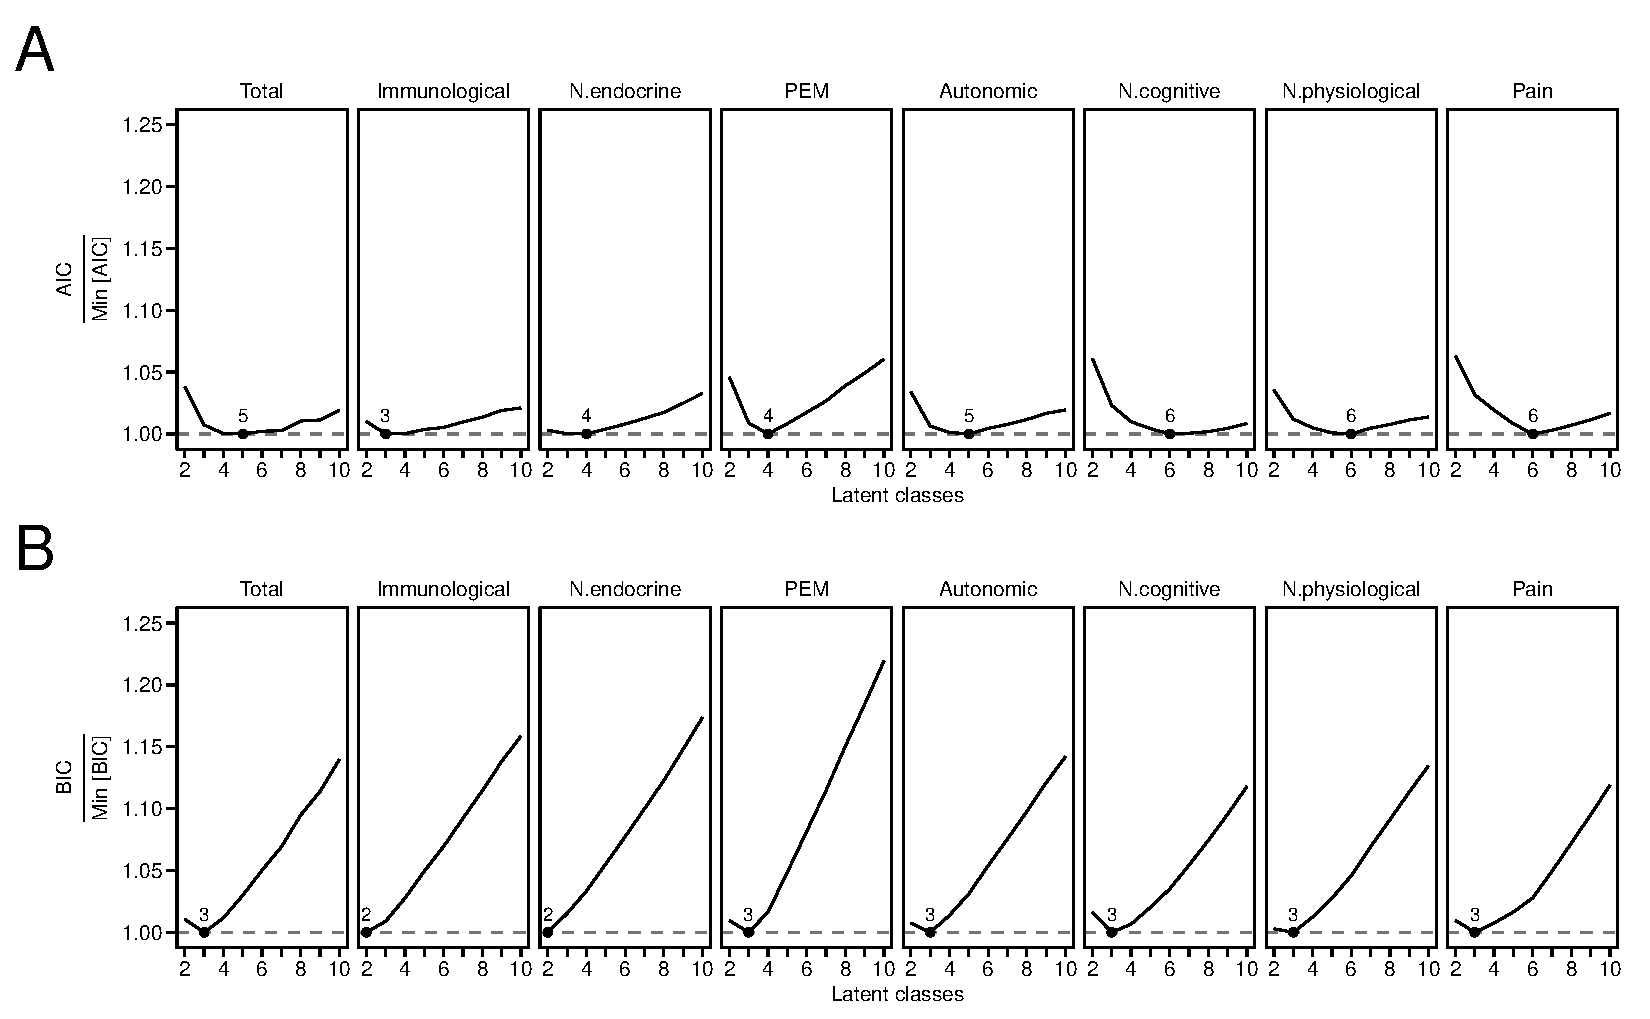
\includegraphics[width=\textwidth]{chapter/2024-sym-domains/figures/fig2-aic-bic-number-of-classes.pdf}
    \caption[Selection of the optimal number of subgroups on each symptomatological domain based on the more parsimonious model]{Selection of the optimal number of subgroups (latent classes) on each symptomatological domain based on the more parsimonious model, considering (A) Akaike information criterion (AIC) or (B) Bayesian information criterion (BIC). For each panel, latent class models were created with the number of subgroups varying between 2 and 10. The results show a standardisation of the estimated AIC and BIC values for each model as a ratio between each original estimated value and with the identified minimum information value as the denominator (black dot at the horizontal dashed line). As a ratio, results closer to 1.00 (the minimal ratio reference) indicate an overall improvement in the estimates for log-likelihood and penalty from the information criteria.}
    \label{fig:fig2-aic-bic-number-of-classes}
\end{figure}
% Figure 3
% Figure~\ref{fig:fig2-aic-bic-number-of-classes}

% ----------------------------------------------------------------------
% differences between AIC & BIC
As detailed in the methodological section, the chosen number of subgroups in each LCA model depends on the applied information criteria.
When comparing the selection outcomes, the information curves resulting from AIC exhibited an overall less pronounced variation, particularly around the optimal number of subgroups.
In other words, the information value varied less while assessing the addition or removal of subgroups.
This variability led to a more distinct number of classes, depending on the considered combination of symptoms, which can be indicative of the patients' large heterogeneity within each domain.
On the other hand, given the more pronounced penalty imposed by BIC for the addition of parameters in the model, the value steadily increased as more than 3 subgroups were taken into consideration.
Consequently, the number of parameters is more homogeneous for the majority of domains.

% ----------------------------------------------------------------------
% AIC
% total
In the analysis encompassing all symptoms, the five AIC-identified subgroups were ordered from g1 to g5, based on the increasing severity of symptoms, according to the LCA class membership probabilities (Figure~\ref{fig:fig3-lca-response-probabilities-aic-total-absent}).
These probability values indicate which combination of symptom severities is more likely to happen in individuals classified into each subgroup.
As such, subgroup g1 classified individuals with higher combinations of absent and mild symptoms, while subgroup g5, at the other extreme, signifies those with class membership probabilities favouring more severe symptoms.
The sample sizes in the subgroups for this domain varied (Table~\ref{tab:tab1-domain-sample-sizes-aic}).
This imbalance was particularly evident in the middle subgroup, g3, which included only 11.62\% of the ME/CFS population (Pearson's $\chi^2$ test, p = 0.007).

\begin{figure}[htbp]
    \centering
    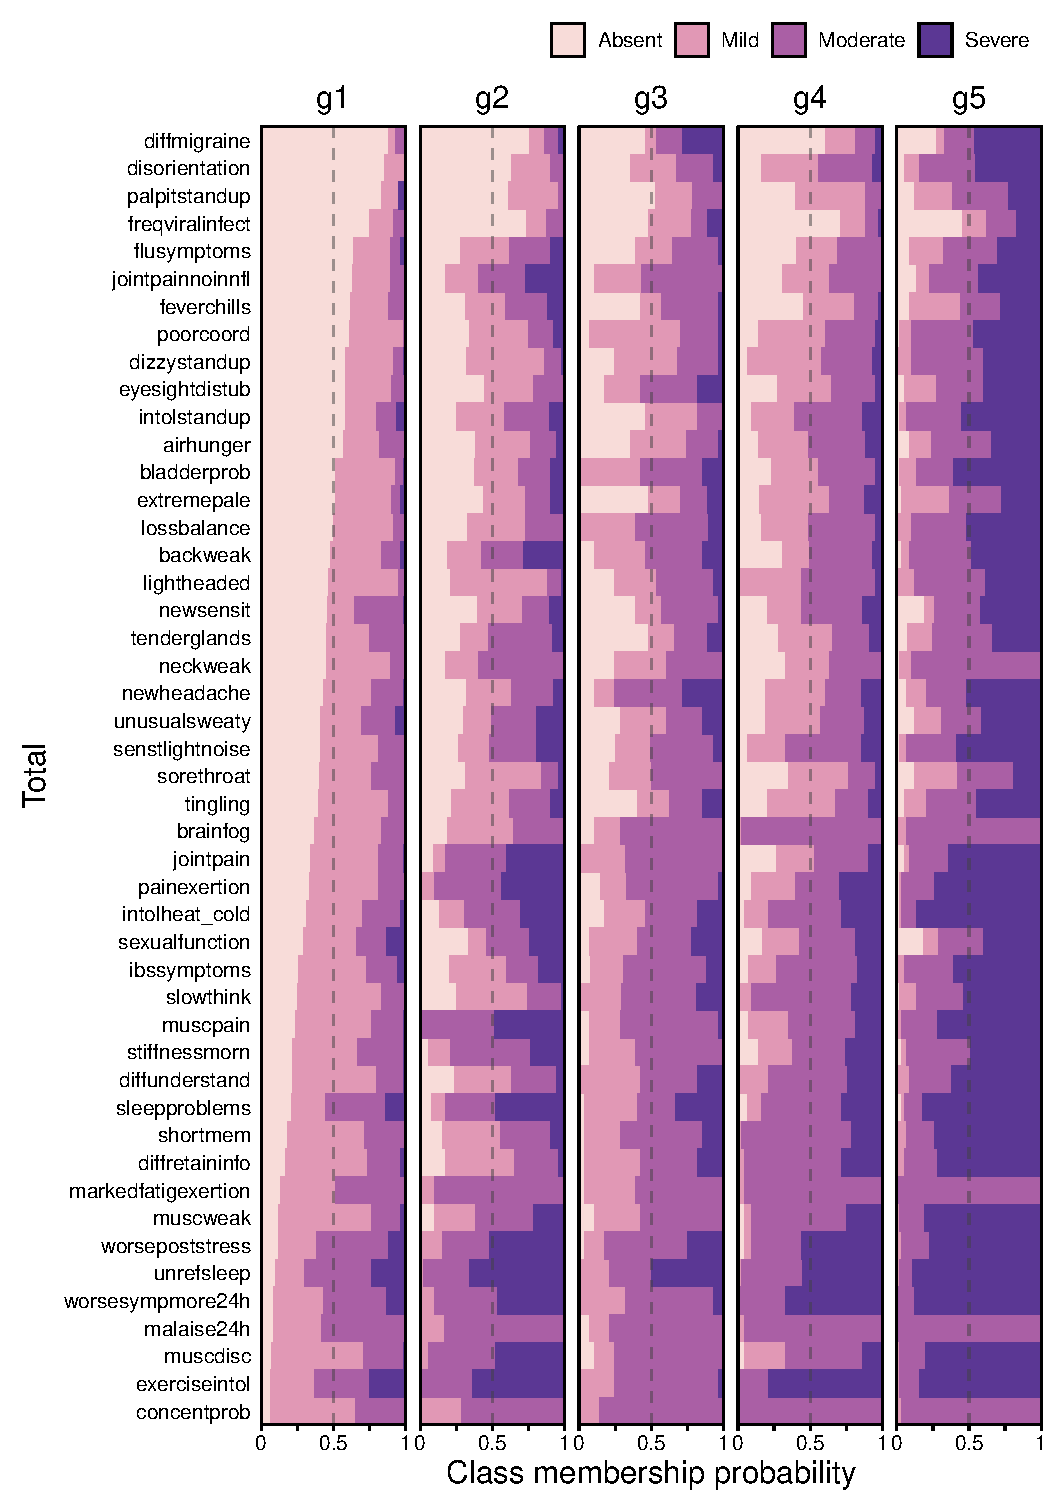
\includegraphics[width=0.9\textwidth]{chapter/2024-sym-domains/figures/fig3-lca-response-probabilities-aic-total-absent.pdf}
    \caption[Latent class analysis estimated class membership probabilities of symptom severities on different AIC-based subgroups, when profiling ME/CFS patients with the totality of available symptoms]{Latent class analysis estimated class membership probabilities of symptom severities on different AIC-based subgroups (latent classes), when profiling ME/CFS patients with the totality of available symptoms. Subgroups were ordered by increasing severity in the response probabilities of symptoms. A more detailed description of each symptom can be found elsewhere (Supplementary Table~\ref{appendix:taba2-sym-description}).}
    \label{fig:fig3-lca-response-probabilities-aic-total-absent}
\end{figure}
% Figure 4
% Figure~\ref{fig:fig3-lca-response-probabilities-aic-total-absent}

\begin{table}[htbp]
    \centering
    \caption[Samples sizes of the 241 ME/CFS patients in each AIC-based latent class estimated on each domain]{Samples sizes (and rounded percentages, row-wise) of the 241 ME/CFS patients in each AIC-based latent class estimated on each domain. For each domain, the latent classes are arranged by increasing level according to the severity profile from the response probabilities (Figure~\ref{fig:fig4-lca-response-probabilities-aic-absent}). Each domain is independent. The optimal number of classes on each domain was chosen based on the Akaike information criterion (AIC). P-values refer to Pearson's $\chi^2$ test.}
    \resizebox{\linewidth}{!}{\begin{tabular}{lccccccc} 
\toprule
\multirow{2}{*}{Domain} & \multicolumn{7}{c}{Latent classes, $n$ (\%)}                                                        \\ 
\cmidrule{2-8}
                        & g1          & g2         & g3         & g4           & g5         & g6         & P-value  \\ 
\midrule
Total                   & 60 (24.90)  & 52 (21.58) & 28 (11.62) & 43 (17.84)   & 58 (24.07) & ---        & 0.007  \\ 
Immunological           & 124 (51.45) & 88 (36.51) & 29 (12.03) & ---          & ---        & ---        & <0.001 \\ 
Neuroendocrine          & 70 (29.05)  & 29 (12.03) & 62 (25.73) & 80 (33.20)   & ---        & ---        & <0.001 \\ 
PEM                     & 6~ (2.49)   & 43 (17.84) & 71 (29.46) & 121 (50.21)  & ---        & ---        & <0.001 \\ 
Autonomic               & 68 (28.22)  & 34 (14.11) & 69 (28.63) & 39 (16.18)   & 31 (12.86) & ---        & <0.001 \\ 
Neurocognitive          & 38 (15.77)  & 50 (20.75) & 34 (14.11) & 31 (12.86)   & 44 (18.26) & 44 (18.26) & 0.279  \\ 
Neurophysiological      & 37 (15.35)  & 19 (7.88)  & 53 (21.99) & 55 (22.82)   & 46 (19.09) & 31 (12.86) & <0.001 \\ 
Pain                    & 38 (15.77)  & 69 (28.63) & 44 (18.26) & 42 (17.43)   & 27 (11.20) & 21 (8.71)  & <0.001 \\
\bottomrule
\end{tabular}}
    \label{tab:tab1-domain-sample-sizes-aic}
\end{table}
% Table 1
% Table~\ref{tab:tab1-domain-sample-sizes-aic}

% by domain
Similar imbalances were observed when performing LCA within specific symptom domains.
The immunological (p < 0.001), neuroendocrine (p < 0.001), and autonomic (p < 0.001) domains had one subgroup close to 12\% of the population, while the PEM (p < 0.001), neurophysiological (p < 0.001), and pain (p < 0.001) domains had one subgroup encompassing less than 10\% of the ME/CFS population.
Only the neurocognitive domain showed a balanced number of individuals across all subgroups (p = 0.279).
In the immunological domain, the majority of patients belonged to the less severe subgroup, g1 ($n = 124$, 51.45\%), whereas the more severe subgroup, g3, comprised the smaller proportion ($n = 29$, 12.03\%).
The neuroendocrine domain had all but subgroup g2 ($n = 29$, 12.03\%) with a sample size above 25\% of the population.
% \red{[neurophysiological description is missing here].}
The autonomic and pain domains showed similar results, classifying a small number of individuals into the more severe subgroup, g5 ($n = 31$, 12.86\%), and g6 ($n = 21$, 8.71\%), respectively.
In contrast, the PEM domain displayed an inverse result, with only six individuals (2.49\%) classified for the g1 subgroup and more than half the population attributed to the more severe cluster g4 ($n = 121$, 50.21\%).
This last outcome could be justified by the requirement of symptoms from this domain for the CCC-2003 clinical diagnosis to be considered valid, explaining the reduced number of individuals classified within this cluster, as the class membership probabilities were mostly for the absent severity (Figure~\ref{fig:fig4-lca-response-probabilities-aic-absent}).

\begin{figure}[htbp]
    \centering
    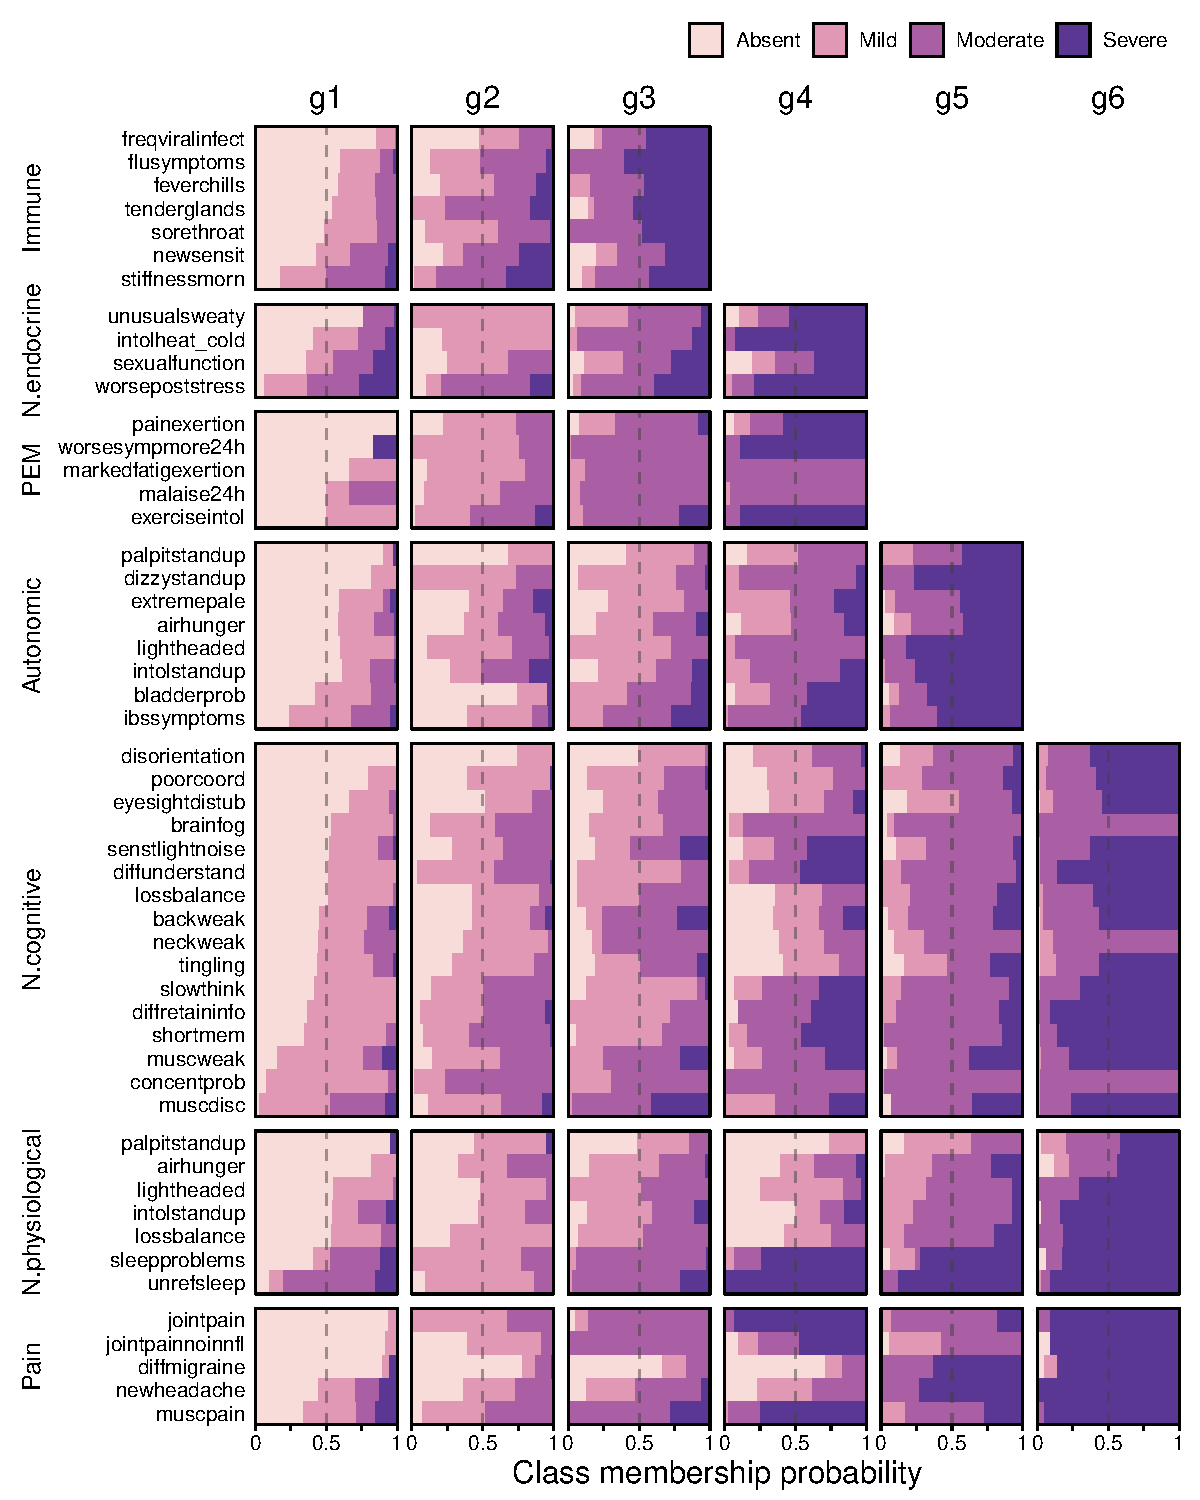
\includegraphics[width=0.9\textwidth]{chapter/2024-sym-domains/figures/fig4-lca-response-probabilities-aic-absent.pdf}
    \caption[Latent class analysis estimated class membership probabilities of symptom severities on different AIC-based subgroups, across the different domains]{Latent class analysis estimated class membership probabilities of symptom severities on different AIC-based subgroups (latent classes), across the different immunological, neuroendocrine, post-exertional malaise (PEM), autonomic, neurocognitive, neurophysiological, and pain domains. Within each domain, subgroups were ordered by increasing severity in the response probabilities of symptoms that make up each domain. A more detailed description of each symptom can be found elsewhere (Supplementary Table~\ref{appendix:taba2-sym-description}).}
    \label{fig:fig4-lca-response-probabilities-aic-absent}
\end{figure}
% Figure 5
% Figure~\ref{fig:fig4-lca-response-probabilities-aic-absent}

\clearpage
% ----------------------------------------------------------------------
% BIC
For the more stringent BIC, the optimal number of latent classes was reduced (Figure~\ref{fig:fig2-aic-bic-number-of-classes}B).
This clarified the association between class membership probabilities and the initially recorded severity level of each symptom (Supplementary Figure~\ref{appendix:figa2-lca-response-probabilities-bic-total-absent} and Supplementary Figure~\ref{appendix:figa3-lca-response-probabilities-bic-absent}).
In contrast to the LCA based on AIC, which identified clusters for a combination of symptoms that gradually increased the severity level over the course of three to six classes, BIC created subgroups based on the profile of absence and mild symptoms in a single group, and mild to severe symptoms in one or more subgroups.
Neuroendocrine, PEM, neurocognitive, and pain domains are examples of this stratification.
Alternatively, this approach allocated an initial subgroup g1, characterised by mostly absent symptoms, while assigning to other groups the presence of symptoms (e.g., g2 in the immunological domain).
Additionally, the latter subgroups could be further stratified into an intermediate group with mild to moderate symptoms and a third one with mostly severe symptoms.
The stratification with all symptoms (Supplementary Figure~\ref{appendix:figa3-lca-response-probabilities-bic-absent}), and the autonomic and neurophysiological domains are examples of this pattern of stratification.
Regarding sample size distribution, there was a significant class imbalance across all domains except the pain domain (Pearson's $\chi^2$ test, p = 0.110) (Supplementary Table~\ref{appendix:taba3-domain-sample-sizes-bic}).
The distributions were in accordance with the AIC-based stratification, most notably in the autonomic domain (p < 0.001), with a smaller number of individuals in the more severe subgroup, g3 ($n = 44$, 18.26\%), and the PEM domain (p < 0.001), with fewer individuals in the initial subgroup, g1 ($n = 45$, 18.67\%).

% Supplementary Table 3
% Supplementary Table~\ref{appendix:taba3-domain-sample-sizes-bic}

% Removal of BIC from the analysis
Further analyses were performed considering the AIC-based latent classes since BIC only identified two to three classes across all domains.
This implies that BIC was essentially distinguishing between an almost binary stratification (absence of symptoms vs. presence of symptoms, regardless of severity, or absence and mild symptoms vs. moderate and severe symptoms), or a stratification which was close to the original one, creating categories for the more extreme situations, absence and more severe cases, with one other category in-between.
% Henceforth, we will describe the results for the AIC LCA models, leaving results based on BIC as supplementary material.


%%%%%%%%%%%%%%%%%%%%%%%%%%%%%%%%%%%%%%%%%%%%%%%%%%%%%%%%%%%%%%%%%%%%%%%%
%%%%%%%%%%%%%%%%%%%%%%%%%%%%%%%%%%%%%%%%%%%%%%%%%%%%%%%%%%%%%%%%%%%%%%%%
\subsection{Herpesvirus IgG antibody data}

% phase 1: KW test
The values of plasma IgG antibodies against the six herpesviruses varied amongst themselves (Figure~\ref{fig:fig5-hc-vs-cfs}A).
There were no significant differences observed when comparing the median antibody values of healthy controls and ME/CFS patients.
However, upon further stratification of patients into distinct domain subgroups, discernible differences emerged (Table~\ref{tab:tab2-serology-pvalues-yhc}).
The (AIC) LCA subgroups identified significant differences in HSV-1 antibody levels within the immunological (Kruskal-Wallis test, p = 0.041, p$_{\text{BH}}$ = 0.285), PEM (p = 0.019, p$_{\text{BH}}$ = 0.068), autonomic (p = 0.002, p$_{\text{BH}}$ = 0.011), and neurocognitive (p = 0.022, p$_{\text{BH}}$ = 0.157) domains.
Other differences were also found in antibody values of herpesvirus HSV-2 in the PEM domain (p = 0.004, p$_{\text{BH}}$ = 0.030), and for herpesvirus EBV VCA within the neurophysiological group of symptoms (p = 0.004, p$_{\text{BH}}$ = 0.030).
Following correction for multiple testing, only the autonomic domain in data from HSV-1, the PEM domain at HSV-2, and neurophysiological in EBV VCA remained.

\begin{figure}[htbp]
    \centering
    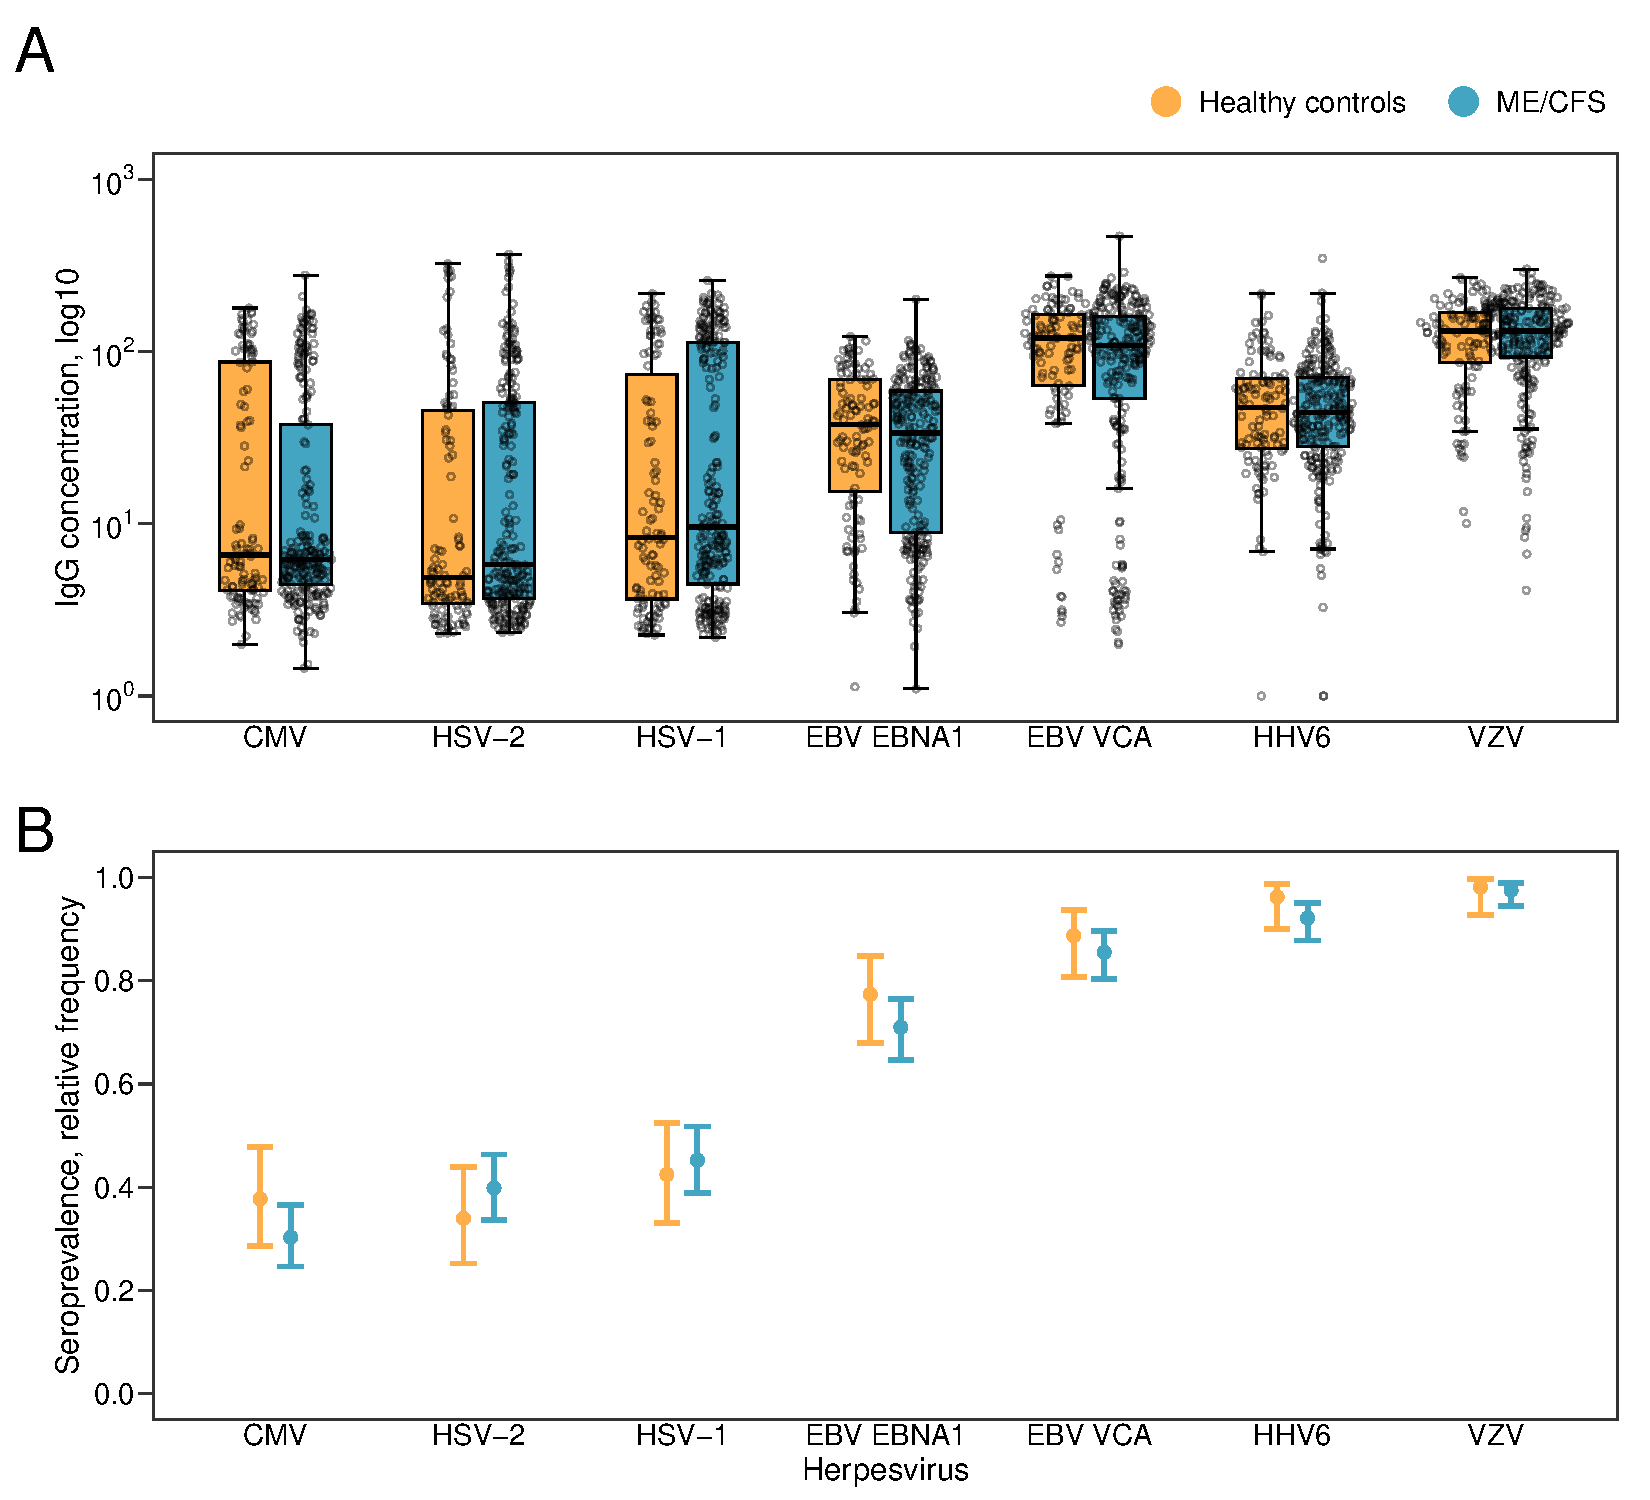
\includegraphics[width=0.9\textwidth]{chapter/2024-sym-domains/figures/fig5-hc-vs-cfs.pdf}
    \caption[Plasma antibody concentrations against herpesviruses and relative seroprevalence in healthy controls and \cfs patients]{Plasma antibody concentrations against herpesviruses and relative seroprevalence in healthy controls and \cfs patients. (A) ${\log_{10}}$-transformed concentration of IgG immunoglobulins reactive against members of the herpesvirus family; (B) Proportion of seropositive individuals in each cohort, with the upper and lower bounds indicating the 95\% CI. Herpesviruses were ordered by the increasing number of seropositive individuals in the data across both cohorts. From a total population of 347 individuals, the number of seropositives were 113 (32.56\%), 132 (38.04\%), 154 (44.38\%), 253 (72.91\%), 300 (86.46\%), 324 (93.37\%), and 339 (97.69\%), respectively for CMV, HSV-2, HSV-1, EBV EBNA1, EBV VCA, HHV6, and VZV.}
    \label{fig:fig5-hc-vs-cfs}
\end{figure}
% Figure 6
% Figure~\ref{fig:fig5-hc-vs-cfs}

\begin{table}[h]
    \centering
    \caption[Selection of significant p-values, both unadjusted and BH-adjusted, from Kruskal-Wallis sum rank test on antibody concentration values across each herpesvirus, comparing different healthy controls and ME/CFS patients under stratification based on symptomatological domains]{Selection of significant p-values, both unadjusted and BH-adjusted, from Kruskal-Wallis sum rank test on antibody concentration values across each herpesvirus, comparing different healthy controls and ME/CFS patients under stratification based on symptomatological domains. p, p-values; p$_{\text{BH}}$, BH-adjusted p-values.}
    \resizebox{\linewidth}{!}{\begin{tabular}{llcccc|cc}
\toprule
Information & Domain & Herpesvirus & Statistic & p & p$_{\text{BH}}$ & \begin{tabular}[c]{@{}c@{}}p, \\new groups\end{tabular} & \begin{tabular}[c]{@{}c@{}}p$_{\text{BH}}$, \\new groups\end{tabular} \\ 
\midrule
AIC & Immunological & HSV-1 & 8.27 & 0.041 & 0.285 & 0.041 & 0.285 \\
 & PEM & HSV-1 & 11.75 & 0.019 & 0.068 & 0.009 & 0.030 \\
 & PEM & HSV-2 & 15.18 & 0.004 & 0.030 & 0.003 & 0.019 \\
 & Autonomic & HSV-1 & 19.54 & 0.002 & 0.011 & <0.001 & 0.002 \\
 & Neurocognitive & HSV-1 & 14.74 & 0.022 & 0.157 & 0.014 & 0.098 \\
 & Neurophysiological & EBV VCA & 18.96 & 0.004 & 0.030 & 0.004 & 0.030 \\
 % & & & & & & \\
BIC & Immune & HSV-1 & 7.73 & 0.021 & 0.146 & --- & --- \\
\bottomrule
\end{tabular}}
    \label{tab:tab2-serology-pvalues-yhc}
\end{table}
% Table 2
% Table~\ref{tab:tab2-serology-pvalues-yhc}


% phase 2: pairwise MW test on significant values
Pairwise tests on the identified herpesvirus-domain associations revealed differences not only between healthy controls and ME/CFS subgroups but also between the subgroups themselves (Figure~\ref{fig:fig6-aic-sero-and-seropos-adj-signif-v2}A).
Disconsidering subgroup g1 in the PEM domain due to its small sample size, there was a significant difference between groups g2 and g3 in the HSV-2 data (Mann-Whitney U test, p = 0.004, p$_{\text{BH}}$ = 0.021).
IgG concentrations for g2 were reduced and g3 (along with g4, albeit not significant post-adjustment) were increased.
The key difference between the two subgroups is that g2 classified individuals with mild PEM symptoms and, given the importance of this domain for the diagnosis of ME/CFS, could be considered as the lowest possible severity values in ME/CFS (with the small group g1 likely being outliers), and g3 mostly classified individuals with a moderate pattern of PEM symptoms (Figure~\ref{fig:fig4-lca-response-probabilities-aic-absent}).
This pattern was also observed in data related to HSV-1, although it was not statistically significant after adjusting for multiple testing.

\begin{figure}[h]
    \centering
    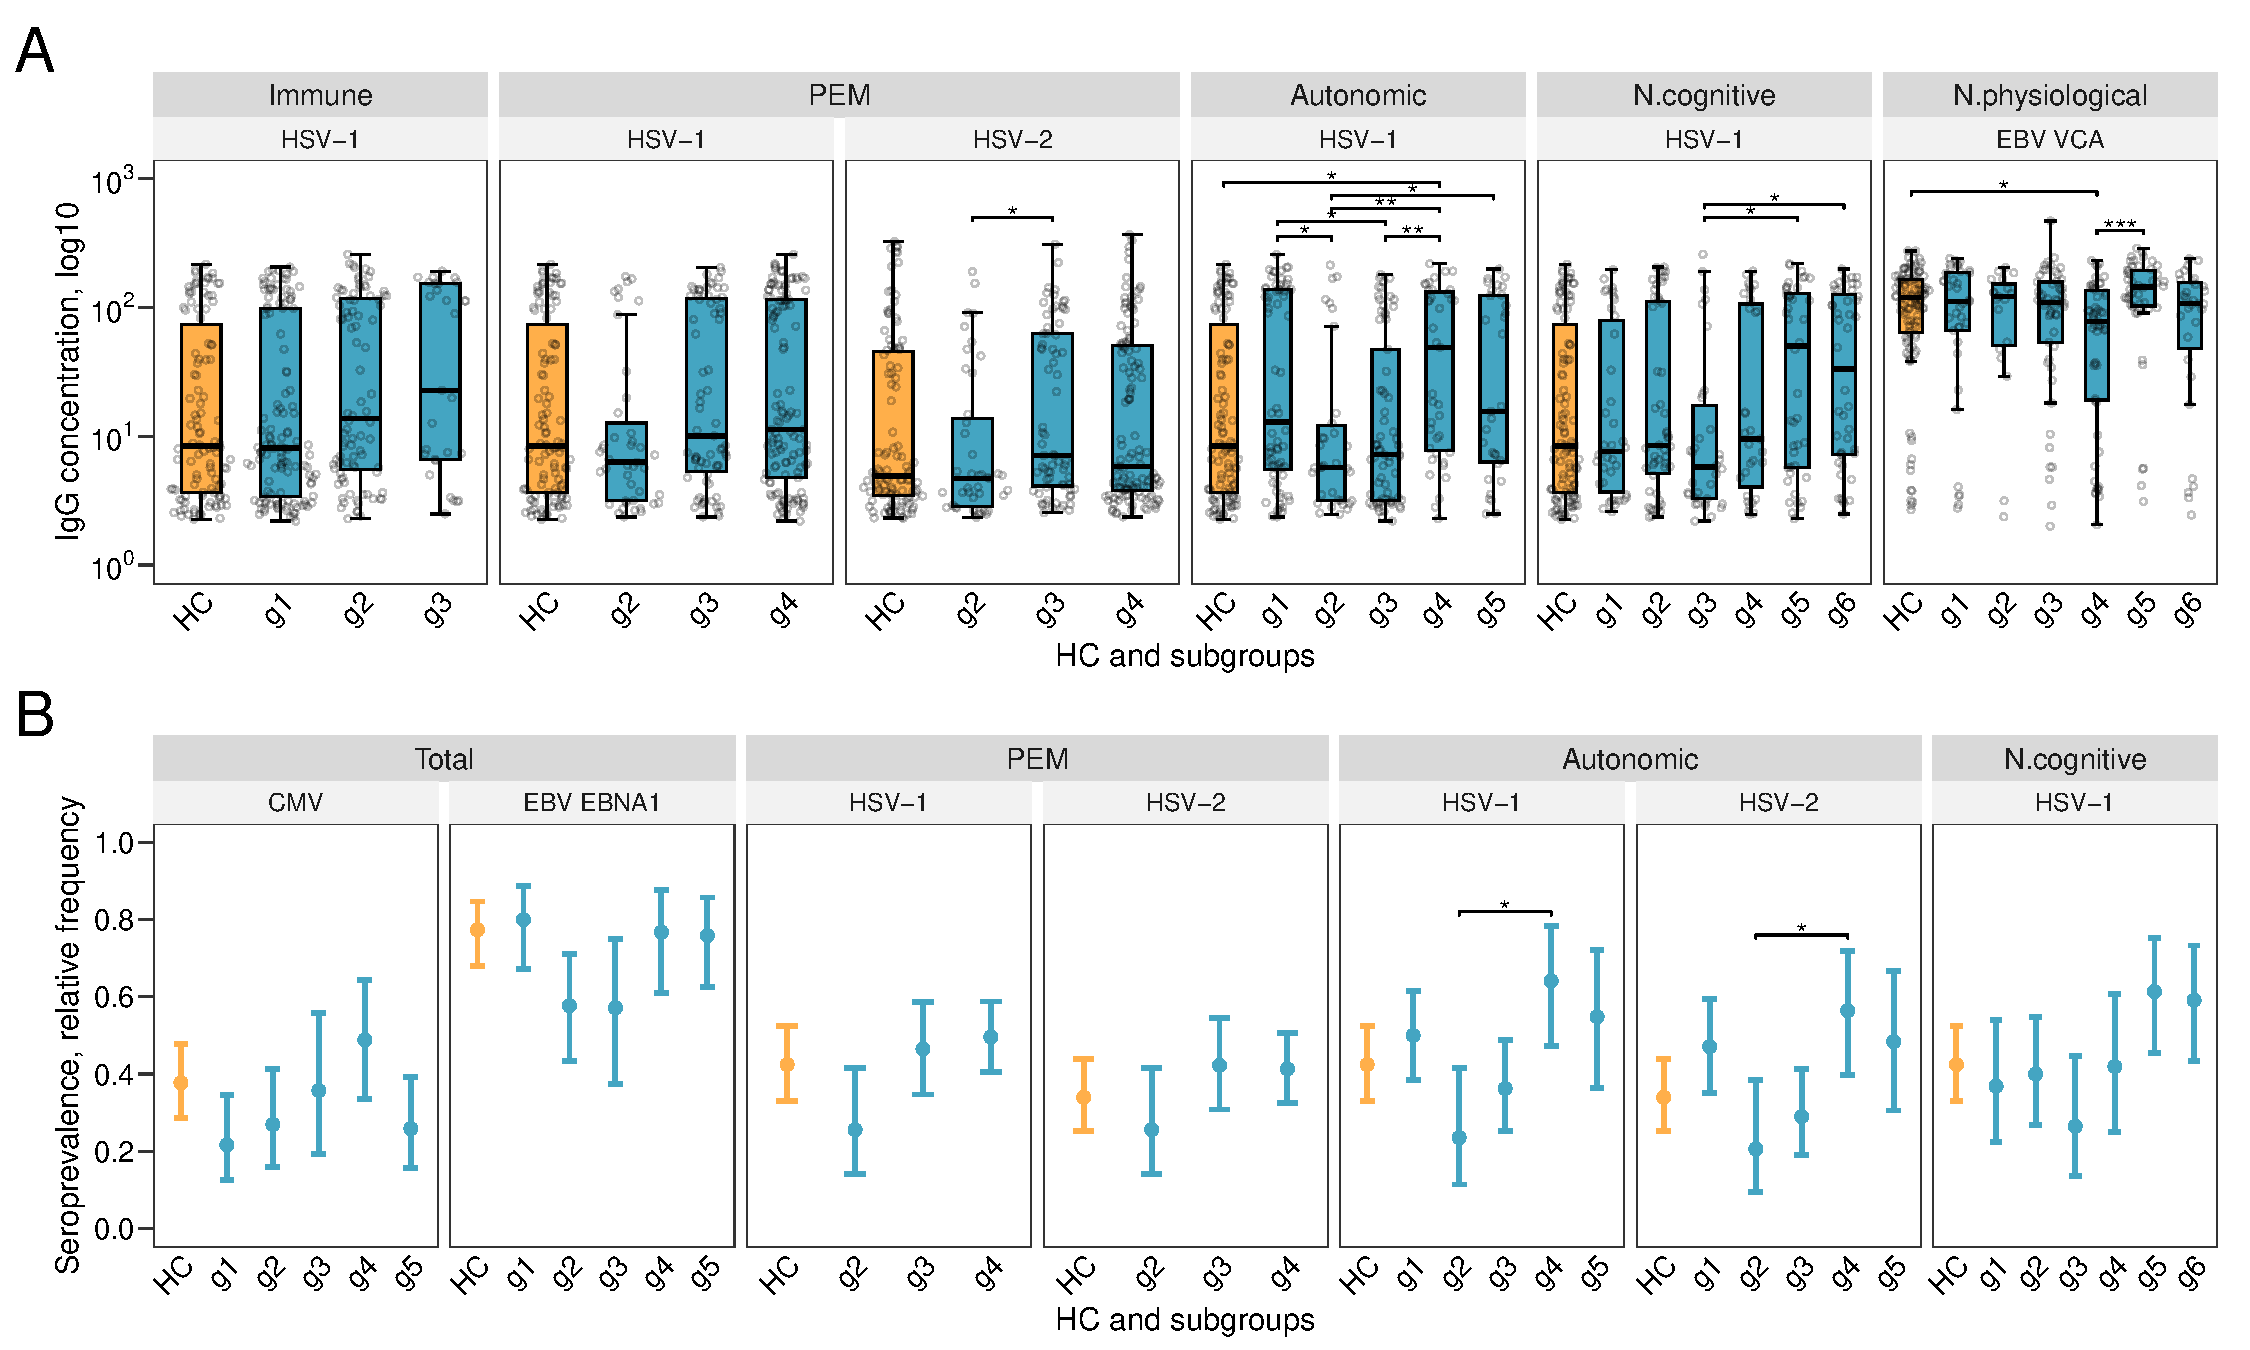
\includegraphics[width=0.95\textwidth]{chapter/2024-sym-domains/figures/fig6-aic-sero-and-seropos-adj-signif-v2.pdf}
    \caption[Plasma antibody concentrations against herpesviruses and relative seroprevalence in healthy controls and subgroups of \cfs patients based on distinct domains]{Plasma antibody concentrations against herpesviruses and relative seroprevalence in healthy controls and subgroups of \cfs patients based on distinct domains. (A) ${\log_{10}}$-transformed concentration of IgG immunoglobulins reactive against members of the herpesvirus family; (B) Proportion of seropositive individuals in each cohort, with the upper and lower bounds indicating the 95\% CI. Significant results from the BH-adjusted pairwise comparisons (Mann-Whitney U test in (A) and Fisher’s exact text in (B)) were given an annotation, with $\ast\ast\ast$ for p < 0.001, $\ast\ast$ when p < 0.01, and $\ast$ when p < 0.05.}
    \label{fig:fig6-aic-sero-and-seropos-adj-signif-v2}
\end{figure}
% Figure 7
% Figure~\ref{fig:fig6-aic-sero-and-seropos-adj-signif-v2}

% autonomic
Various differences were observed in the subgroups of the autonomic domain on HSV-1 data.
Most notably, reduced concentrations for subgroups g2 and g3, and increased values for subgroup g4.
Subgroups g2 and g3 had similar median concentration levels and differed significantly when compared to g4 (g2, p = 0.001, p$_{\text{BH}}$ = 0.008; g3, p = 0.001, p$_{\text{BH}}$ = 0.008).

% neurocognitive
In the neurocognitive domain in HSV-1, the pairwise analyses identified a reduction in subgroup g3 when compared to the two more severe subgroups, g5 (p = 0.003, p$_{\text{BH}}$ = 0.036) and g6 (p < 0.002, p$_{\text{BH}}$ = 0.036).
% Similarly, the BIC stratification of the immunological domain also identified a significant increase in antibodies against HSV-1 in the more severe subgroup g2 when compared to both healthy controls (p = 0.020, p$_{\text{BH}}$ = 0.030) and g1 (p = 0.011, p$_{\text{BH}}$ = 0.030).
% These results suggested potential associations between specific herpesviruses and different symptom domains.

% neurophysiological
Lastly, subgroup g4 from the neurophysiological domain showed reduced antibody concentrations when compared to both healthy controls (p = 0.004, p$_{\text{BH}}$ = 0.037) and the group g5 (p < 0.001, p$_{\text{BH}}$ = 0.001).
This particular group classified few individuals with moderate symptoms, presenting a distinct profile characterised by almost exclusively severe levels in the two symptoms related to sleep dysfunction (sleepproblems and unrefsleep) and absent to mild severity levels for the remaining five symptoms (palpitstandup, airhunger, lightheaded, intelstandup, and lossbalance) (Figure~\ref{fig:fig4-lca-response-probabilities-aic-absent}).
The observed differences towards healthy controls could be attributed to increased problems with sleep dysfunction, while the differences towards g5 could be linked to reduced severity in the other symptoms, as patients from this group also exhibit severe levels of sleep-related symptoms.

% ----------------------------------------------------------------------
% ----------------------------------------------------------------------
\bsni
% Group specific subgroups together
We then merged neighbouring pairs of domain subgroups that were closely related in terms of antibody concentration levels.
With this, our intent was to reduce the uncertainty that could arise from working with groups of smaller sample sizes.
% , which would make the initially identified patterns more consistent.
The pairs formed were subgroups g3--g4 from the PEM domain, subgroups g2--g3 and g4--g5 from the autonomic domain, and subgroups g3--g4 and g4--g5 from the neurocognitive domain (Table~\ref{tab:tab2-serology-pvalues-yhc}, Figure~\ref{fig:fig7-aic-sero-and-seropos-adj-signif-merged-v2}A).

% \red{[should mention the results for Pearson's $\chi^2$, or go straight to the pairwise comparisons? The results are pretty much the same (were added in a table)]}.
This grouping strategy kept relevant the strong differences initially noted in the HSV-1 antibody concentration levels for the autonomic domain (Kruskal-Wallis test, p < 0.001, p$_{\text{BH}}$ = 0.002) 
and the 
% neurocognitive domain (p = 0.014, p$_{\text{BH}}$ = 0.098), as well as the 
PEM domain at the HSV-2 levels (p = 0.003, p$_{\text{BH}}$ = 0.019) (Table~\ref{tab:tab2-serology-pvalues-yhc}).
Interestingly this approach also evidenced differences in the PEM domain for the HSV-1 (p = 0.009, p$_{\text{BH}}$ = 0.019).
% , which in the same domain presented a similar pattern to the HSV-2 data.
In this domain, the subgroup g3--g4 of moderate to severe \cfs patients consistently reported higher concentrations of antibodies, differing from subgroup g2, with noticeably lower concentrations (Mann-Whitney U test, HSV-1, p = 0.010, p$_{\text{BH}}$ = 0.046; HSV-2, p = 0.008, p$_{\text{BH}}$ = 0.023) (Figure~\ref{fig:fig7-aic-sero-and-seropos-adj-signif-merged-v2}A).

In the autonomic domain, HSV-1 concentrations exhibited similar results, more clearly relating the increase of symptom severity (subgroup g4--g5) with an increase in antibody concentrations, comparatively to healthy individuals (p = 0.005, p$_{\text{BH}}$ = 0.011) and to subgroup g2--g3 (p < 0.001, p$_{\text{BH}}$ < 0.001).

In the neurocognitive domain, the more severe subgroup g5--g6 also showed a significant increase in antibody concentrations for the same herpesvirus when compared to healthy controls (p = 0.005, p$_{\text{BH}}$ = 0.021).

\begin{figure}[h]
    \centering
    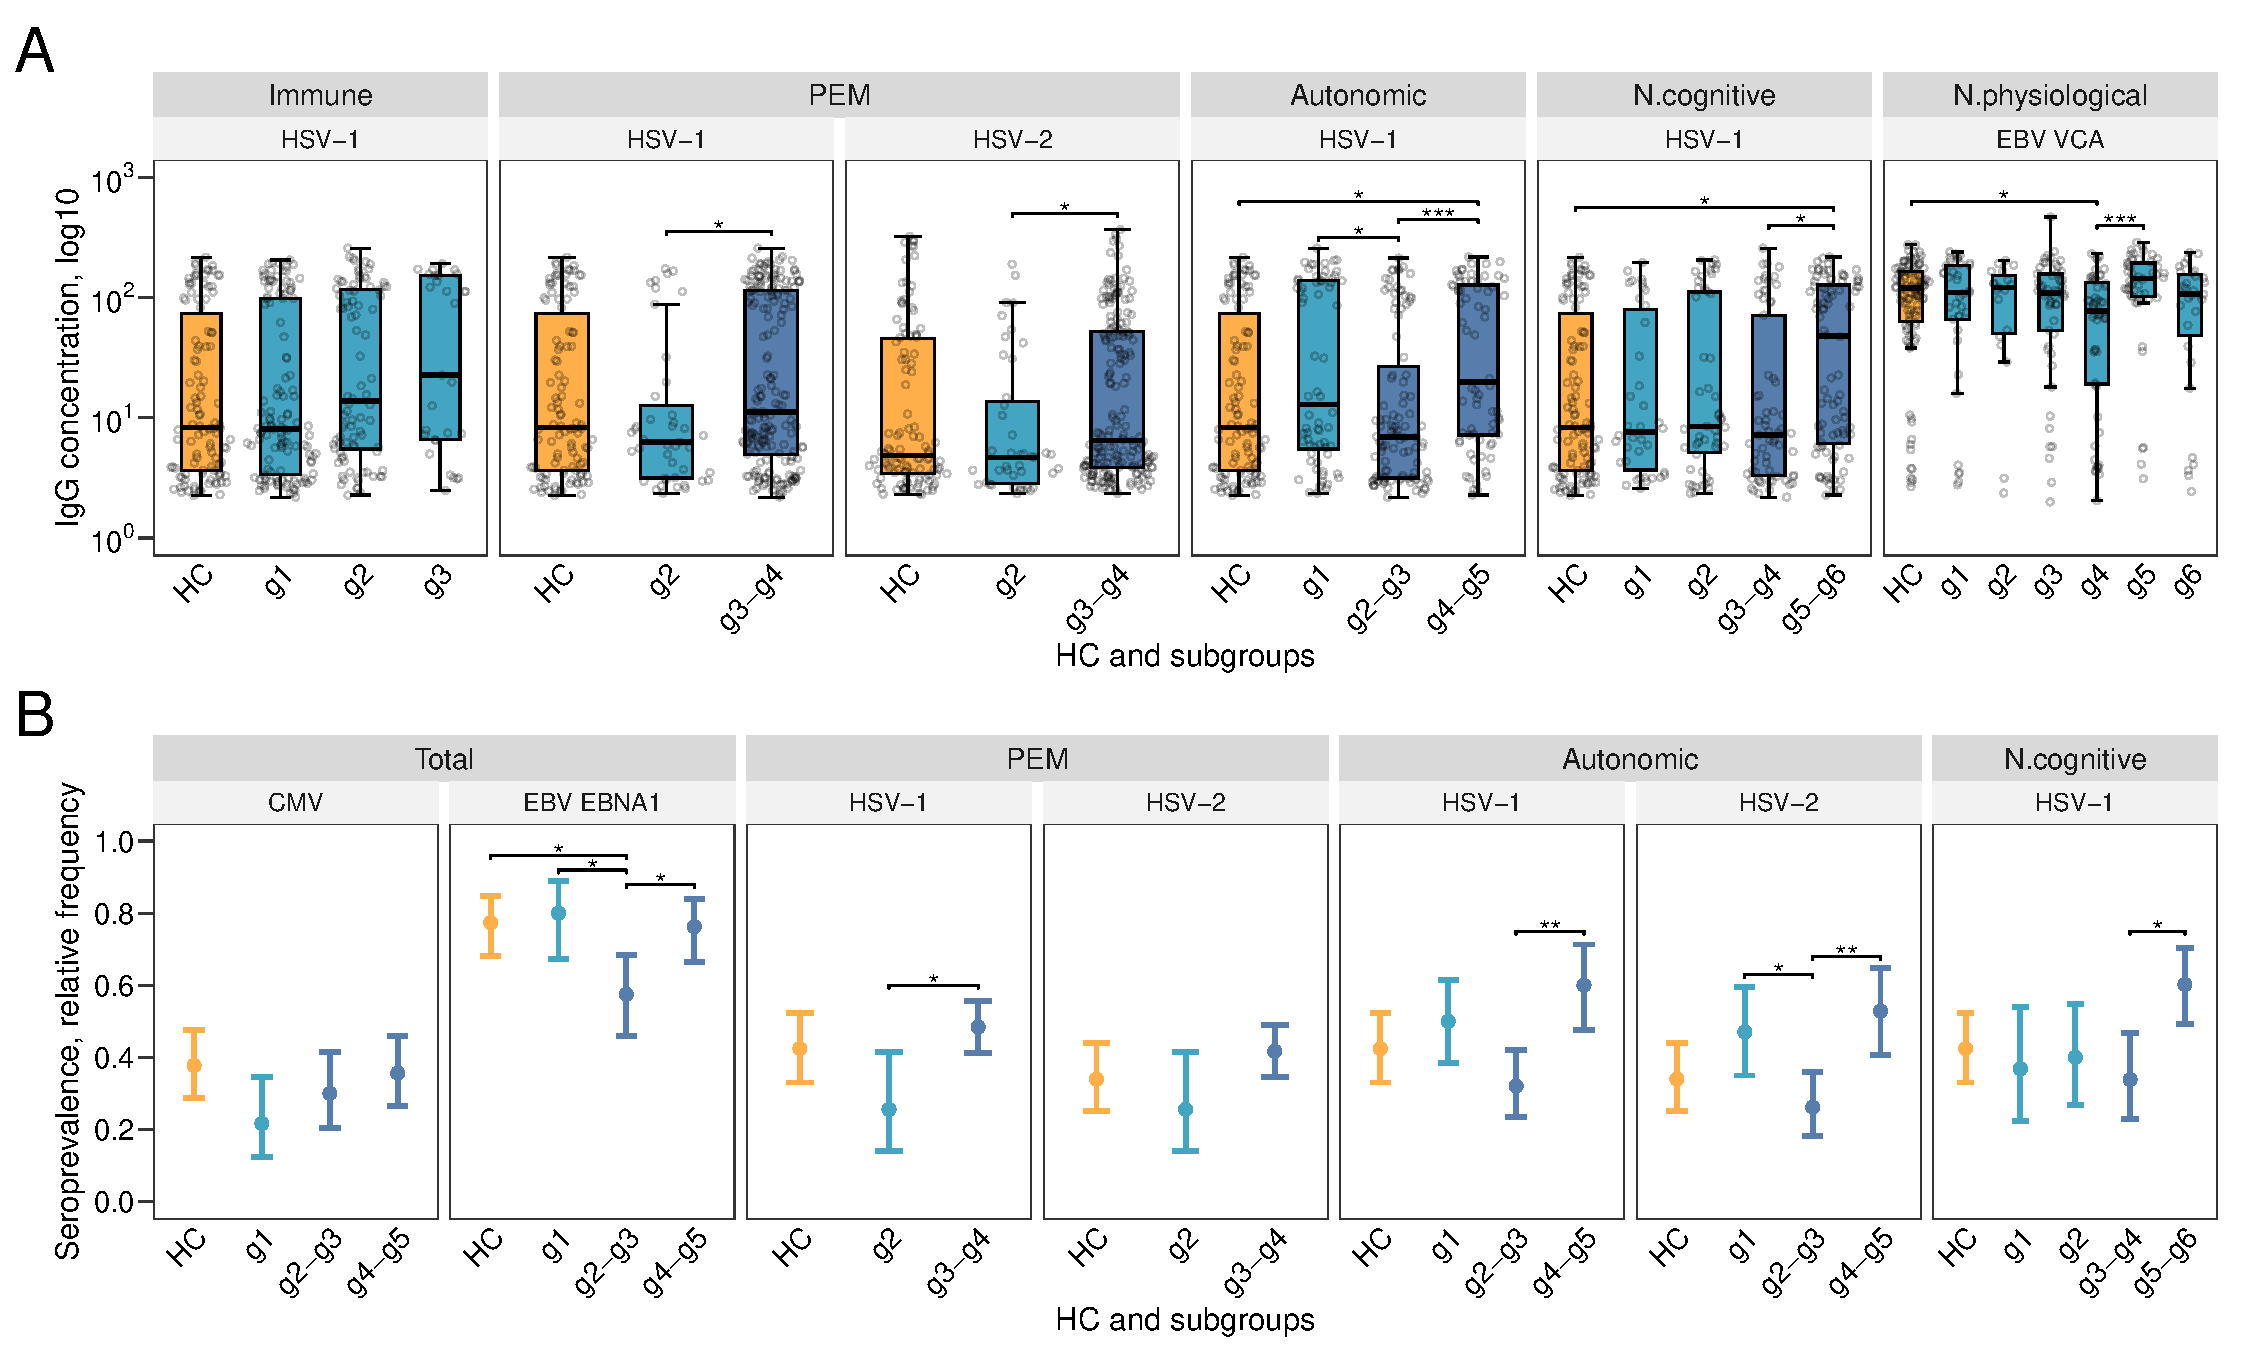
\includegraphics[width=0.95\textwidth]{chapter/2024-sym-domains/figures/fig7-aic-sero-and-seropos-adj-signif-merged-v2.pdf}
    \caption[Plasma antibody concentrations against herpesviruses and relative seroprevalence in healthy controls and homogenised \cfs subgroups of patients based on distinct domains]{Plasma antibody concentrations against herpesviruses and relative seroprevalence in healthy controls and homogenised \cfs subgroups of patients based on distinct domains. (A) ${\log_{10}}$-transformed concentration of IgG immunoglobulins reactive against members of the herpesvirus family; (B) Proportion of seropositive individuals in each cohort, with the upper and lower bounds indicating the 95\% CI. Significant results from the BH-adjusted pairwise comparisons (Mann-Whitney U test in (A) and Fisher’s exact text in (B)) were given an annotation, with $\ast\ast\ast$ for p < 0.001, $\ast\ast$ when p < 0.01, and $\ast$ when p < 0.05.}
    \label{fig:fig7-aic-sero-and-seropos-adj-signif-merged-v2}
\end{figure}
% Figure 7
% Figure~\ref{fig:fig7-aic-sero-and-seropos-adj-signif-merged-v2}

%%%%%%%%%%%%%%%%%%%%%%%%%%%%%%%%%%%%%%%%%%%%%%%%%%%%%%%%%%%%%%%%%%%%%%%%
%%%%%%%%%%%%%%%%%%%%%%%%%%%%%%%%%%%%%%%%%%%%%%%%%%%%%%%%%%%%%%%%%%%%%%%%
\subsection{Herpesvirus seropositivity}

% Phase 2: Pearson's $\chi^2$ test
The differences observed in the herpesviruses' serology influenced the seroprevalence in the study populations (Figure~\ref{fig:fig5-hc-vs-cfs}B, HC vs. ME/CFS across herpesviruses).
Similarly to the previous section, the comparison between healthy controls and \cfs patients showed consistent results across all herpesviruses.
However, following the stratification of ME/CFS into the seven specific domains, differences became more apparent (Table~\ref{tab:tab3-seroprevalence-pvalues-yhc}).
In line with the results obtained when studying antibody titers, the AIC-based subgroups showed significant differences in HSV-1 seroprevalence in the PEM (Pearson's $\chi^2$ test, p = 0.022, p$_{\text{BH}}$ = 0.148), autonomic (p = 0.006, p$_{\text{BH}}$ = 0.020), and neurocognitive in HSV-1 (p = 0.021, p$_{\text{BH}}$ = 0.146) domains.
Differences in HSV-2 seroprevalence in the PEM domain (p = 0.042, p$_{\text{BH}}$ = 0.148) were also observed.
Other significant differences appeared, namely in the stratification considering all symptoms across CMV (p = 0.038, p$_{\text{BH}}$ = 0.132) and EBV EBNA1 (p = 0.025, p$_{\text{BH}}$ = 0.132), and autonomic domain at the HSV-2 herpesvirus (p = 0.005, p$_{\text{BH}}$ = 0.020).
% Subgroups created by the BIC only identified a relation between the neuroendocrine domain and the HHV6 herpesvirus prevalence values (p = 0.016, p$_{\text{BH}}$ = 0.115).
After correction for multiple testing, all previously significant results were disregarded with the exception of the autonomic relations within prevalence values for the two herpes simplex viruses.
% members of the human \textit{Herpesviridae} family.

\begin{table}[h]
    \centering
    \caption[Selection of significant p-values, both unadjusted and BH-adjusted, from Pearson's $\chi^2$ test on seropositivity values across each herpesvirus, comparing different healthy controls and ME/CFS patients under stratification based on symptomatological domains]{Selection of significant p-values, both unadjusted and BH-adjusted, from Pearson's $\chi^2$ test on seropositivity values across each herpesvirus, comparing different healthy controls and ME/CFS patients under stratification based on symptomatological domains. p, p-values; p$_{\text{BH}}$, BH-adjusted p-values.}
    \resizebox{\linewidth}{!}{\begin{tabular}{llcccc|cc}
\toprule
Information & Domain & Herpesvirus & Statistic & p & p$_{\text{BH}}$ & \begin{tabular}[c]{@{}c@{}}p, \\new groups\end{tabular} & \begin{tabular}[c]{@{}c@{}}p$_{\text{BH}}$, \\new groups\end{tabular} \\ 
\midrule
AIC & Total & CMV & 11.79 & 0.038 & 0.132 & --- & --- \\
& Total & EBV EBNA1 & 12.79 & 0.025 & 0.132 & 0.005 & 0.036 \\
% & PEM & HHV6 & 8.34 & — & — & 0.040 & 0.092 \\
& PEM & HSV-1 & 11.46 & 0.022 & 0.148 & 0.010 & 0.069 \\
& PEM & HSV-2 & 9.89 & 0.042 & 0.148 & 0.020 & 0.069 \\
& Autonomic & HSV-1 & 16.39 & 0.006 & 0.020 & 0.003 & 0.009 \\
& Autonomic & HSV-2 & 16.88 & 0.005 & 0.020 & 0.001 & 0.009 \\
& Neurocognitive & HSV-1 & 14.91 & 0.021 & 0.146 & 0.010 & 0.069 \\
BIC & Neuroendocrine & HHV6 & 8.22 & 0.016 & 0.115 & --- & --- \\
\bottomrule
\end{tabular}}
    \label{tab:tab3-seroprevalence-pvalues-yhc}
\end{table}
% Table 3
% Table~\ref{tab:tab3-seroprevalence-pvalues-yhc}

% Phase 2: Pairwise comparisons
Pairwise comparisons on the autonomic results were in line with the ones seen in the previous section (see Figure~\ref{fig:fig6-aic-sero-and-seropos-adj-signif-v2}A), showing reduced seroprevalence values on subgroups g2 and g3 overall (Figure~\ref{fig:fig6-aic-sero-and-seropos-adj-signif-v2}B).
Other results on both HSV-1 and HSV-2 were the noticeable seroprevalence similarities between the two more severe groups, g4 and g5.
This could explain a relation between past exposure to HSV-1 (and/or HSV-2) and the development of more pronounced autonomic symptoms.
In the neurocognitive domain, the more severe subgroups, g5 and g6, also showed higher seroprevalence, albeit not significant.
% , on both HSV-1 and HSV-2 and the same elevated pattern for the two more severe subgroups, g5 and g6, also on HSV-1.

\bsni
% Group specific subgroups together
As previously, we merged groups with similar seroprevalence estimates.
In line with the serological section, the subgroup pairs were g3--g4 from the PEM domain, pairs g2--g3 and g4--g5 from the autonomic domain, and pairs g3--g4 and g5--g6 from the neurocognitive domain (Figure~\ref{fig:fig7-aic-sero-and-seropos-adj-signif-merged-v2}B).
Two additional pairs were formed for the stratification with all symptoms, g2--g3, and g4--g5.
From this, only the seroprevalence values for EBV EBNA1 when clustering for all symptoms yielded a new relation (p = 0.005, pBH = 0.036) (Table~\ref{tab:tab3-seroprevalence-pvalues-yhc}), which showed a seroprevalence reduction in the intermediate group g2--g3 when compared to healthy controls and remaining \cfs subgroups.
On par with the HSV-1 IgG concentration values, seroprevalence was also higher in the more severe subgroup g3--g4 from the PEM domain, subgroup g4--g5 from the autonomic domain, and subgroup g5--g6 from the neurocognitive domain.
% 3.x Predicting seropositivity based on LCA posterior probabilities?


%%%%%%%%%%%%%%%%%%%%%%%%%%%%%%%%%%%%%%%%%%%%%%%%%%%%%%%%%%%%%%%%%%%%%%%%
%%%%%%%%%%%%%%%%%%%%%%%%%%%%%%%%%%%%%%%%%%%%%%%%%%%%%%%%%%%%%%%%%%%%%%%%
%%%%%%%%%%%%%%%%%%%%%%%%%%%%%%%%%%%%%%%%%%%%%%%%%%%%%%%%%%%%%%%%%%%%%%%%
\section{Discussion}

% heterogeneity within patients
This preliminary study demonstrates how the wide range of symptoms assessed during \cfs diagnosis could be used to stratify patients by mechanistic domains.
% of ME/CFS can ultimately create a heterogeneous group of patients that is categorised with the same disease.
% - Establishing consensus on ME/CFS \citep{jason2023EstablishingConsensus}
% - d heterogeneity of symptoms 
% - challenging it is to 

% ----------------------------------------------------------------------
% intra- and inter-rater analysis
The findings from the intra- and inter-rater agreement analyses indicated that patients diagnosed with \cfs are quite diverse in terms of symptom severity, both at the individual and population levels (Figure~\ref{fig:fig1-id-entropy-and-mds}).
Similar to the symptom-based case definitions, the severity profile from all individuals distinguished healthy controls from patients (absence vs. presence of disease) and identified clusters of patients with consistently increased levels of symptom severity (mild to moderate vs. severely affected).
Stratification based on this binary phenotype for mild vs. severe \cfs has been previously studied and even used to research the link between the disease and herpesviruses, using data from the UKMEB \citep{cliff2019CellularImmune, lee2021SalivaryDNA}.
For instance, \citet{lee2021SalivaryDNA} found a positive correlation between the HHV6 viral load and higher severity scores from symptoms in the autonomic, neurocognitive, and pain domains.
% However, the phenotype for severe \cfs has already been described, with few differences reported in serological and immunological data \citep{cliff2019CellularImmune}.
% Our results showed that not only individuals experience widely heterogeneous patterns of severity among the assessed symptoms (entropy levels close to the maximum possible value, Figure~\ref{fig:fig1-id-entropy-and-mds}A), but also the symptomatological profile varies between patients (Figure~\ref{fig:fig1-id-entropy-and-mds}B).

% ----------------------------------------------------------------------
% LCA in all 
The LCA method allowed us to test an unbiased approach to symptom-based clustering based on pre-specified domains.
When dividing all symptoms into subgroups, the two more extreme groups, g1 and g5, showed clearer profiles of more absent and mild, and more severe symptoms, respectively (Figure~\ref{fig:fig3-lca-response-probabilities-aic-total-absent}).
The remaining three subgroups showed a combination of gradually increasing severity in most symptoms.
Interestingly, g1 and g5 included a similar number of patients and together accounted for almost half the \cfs population.

It is worth noting that PEM and sleep-related symptoms (exerciseintol, malaise24h, markedfatigexertion, painexertion, and worsesympmore24h, and sleepproblems and unrefsleep, respectively) were the only ones where the sum of class membership probability estimates from mild and severe surpassed the estimated class membership probabilities midpoint value of 0.5 on all five subgroups, being particularly evident in subgroup g1.
This highlights the importance of both PEM and sleep disturbances in order to comply with the case diagnosis---the presence of symptoms from the two domains are requirements for the CCC-2003 case definition and are listed as necessary in the CDC-1994 \citep{fukuda1994ChronicFatigue, carruthers2003MyalgicEncephalomyelitis}.

The analysis of serological data using patients split by these five subgroups did not yield conclusive results.
Similar to the comparisons using the entire \cfs population, we did not find any significant differences in either antibody concentrations or seroprevalence comparisons.
After combining two subgroups (moderate subgroup g2--g3 and severe subgroup g4--g5), we found a significant decrease in seroprevalence in the moderate group for EBV EBNA1 (Figure~\ref{fig:fig7-aic-sero-and-seropos-adj-signif-merged-v2}B).
However, this decrease in the intermediate subgroup g2--g3 does not provide much information.
Nonetheless, it is still noteworthy that g2--g3 consistently showed a far lower percentage of seropositive individuals (57.50\%, 95\% CI = [45.95\%, 68.32\%]) when the overall 70.95\% (95\% CI = [64.71\%, 76.51\%]) of the \cfs population is seropositive towards EBV EBNA1 (Figure~\ref{fig:fig5-hc-vs-cfs}B).

% \bsni
% ----------------------------------------------------------------------
% LCA in specific domains
When implementing the LCA method over specific symptom domains, the optimal number of subgroups varied (Figure~\ref{fig:fig2-aic-bic-number-of-classes}A).
This suggests that there are different degrees of symptom heterogeneity within each domain.
In some, patients are more similar and show fewer subgroups, such as the immunological, neuroendocrine, and PEM domains.
Conversely, in the pain, neurophysiological, and neurocognitive domains, \cfs patients exhibit a more heterogeneous profile of symptoms, resulting in a larger number of optimal latent classes (Figure~\ref{fig:fig4-lca-response-probabilities-aic-absent}).
% While both pain and neurocognitive domains
% , some differences became clearer.
One example of the latter is the pain domain, where distinct subgroups conveyed clear profiles of symptom severity.
Subgroup g4 classified individuals with severe muscle and multi-joint pain, and subgroup g5 identified individuals reporting severe headaches and migraines together with a moderate level of physical joint and muscle pain.
Lastly, subgroup g6 almost exclusively included patients experiencing severe symptoms.
Since severe chronic pain greatly reduces the overall well-being and quality of life, there are pharmacological therapies listed as recommendations to relieve pain in \cfs \citep{niceguideline2021OverviewMyalgic}.
As such, it makes sense that this was the smaller subgroup from this domain (Table~\ref{tab:tab1-domain-sample-sizes-aic}).
% where there was a reduced number of \cfs individuals observed with maximal severity of symptoms (subgroup g6 in Table~\ref{tab:tab1-domain-sample-sizes-aic}).

% ----------------------------------------------------------------------
% adding serology
% HSV1
% Crossing the domain subgroups with serological data showed 
Similar to the previous analysis, IgG concentrations in conjunction with domain subgroups did not reveal a clear relationship between severity and antibody titers.
Overall, the most significant differences were observed for HSV-1, particularly in the autonomic and neurocognitive domains (Figure~\ref{fig:fig6-aic-sero-and-seropos-adj-signif-v2}A).
In the autonomic domain, individuals in subgroup g4 had higher antibody levels compared to those in intermediate subgroups, g2 and g3, and healthy controls.
Similarly, within the neurocognitive domain, high antibody levels against HSV-1 were observed in the severe groups, g5 and g6, in comparison to the intermediate g3.
When combining the subgroups, the differences between the more severe (g4--g5 in the autonomic and g5--g6 in the neurocognitive domain) and healthy controls became more pronounced (Figure~\ref{fig:fig7-aic-sero-and-seropos-adj-signif-merged-v2}A).
Interestingly, the seroprevalence results also showed an increased number of HSV-1 seropositive individuals in the more severe groups of autonomic and neurocognitive domains (Figure~\ref{fig:fig6-aic-sero-and-seropos-adj-signif-v2}B and Figure~\ref{fig:fig7-aic-sero-and-seropos-adj-signif-merged-v2}B).
This observation could be attributed to the neurotropic nature of the virus \citep{olsson2016HSVPresence, marcocci2020HerpesSimplex}, as there is evidence that repeated HSV-1 brain infections can lead to neuronal damage \citep{marcocci2020HerpesSimplex, murphy2021HerpesSimplex}.
However, the inferences regarding positive associations between autonomic and neurocognitive subgroup severity and serological measures for HSV-1 are not so linear.
In both domains, subgroups classified as mostly absent to mild (g1 in autonomic, and g1 and g2 in neurocognitive) did not showed minimal levels of antibody concentrations or seroprevalence.
One speculative explanation could be that these subgroups are closer to healthy controls in terms of symptoms and HSV-1 serological values.
However, to confirm this hypothesis would require the individuals from both domains to be the same, and looking at the profile of each individual across all domains was not in the scope of this preliminary study.
Nonetheless, despite the lack of concrete interpretations, this intriguing result should be further explored in subsequent works.

% HSV2
The seroprevalence results for the autonomic domains in HSV-1 were also observed in HSV-2.
This correlated result could be influenced by the close relation between the two herpes simplex viruses, as they share similarities in terms of their structure, transmission methods, and symptoms caused \citep{bradley2014SeroprevalenceHerpes, kawaguchi2018HumanHerpesviruses}.

% EBV

\bsni
% \subsubsection{Combinatorial analysis}
% ----------------------------------------------------------------------
% combinatorial analysis study
The motivation behind this approach stems from the need to simplify the myriad of potential symptom combinations across the \cfs population.
Conceptually, this task could be viewed as a combinatorial problem.
To begin, we consider an extreme scenario under two assumptions: (1) there are no constraints from the usual case definitions used to diagnose \cfs, implying that patients 
% are characterised \textit{a priori} and 
can experience any symptom at any range (absent, mild, moderate, or severe); and (2) the 47 assessed symptoms are independent of each other, meaning that the manifestation of one symptom does not influence the occurrence of another potentially related one.

Under these assumptions, the number of distinct and possible symptom profiles would be $4^{47} = 1.98 \times 10^{28}$.
Certainly, many of these profiles consist of combinations predominantly featuring absence to mild symptoms, or only a small number of exacerbated and isolated symptoms, insufficient to comply with a comprehensive \cfs diagnosis.
However, even after removing those less relevant combinations for absent and sporadic symptoms, and reconsidering the previous assumptions of symptom independence and case criteria restrictions, the number of possible combinations would still be immeasurable.

The act of grouping symptoms into specific domains offers a means to mitigate this complexity, simplifying the vast number of potential combinations into a more perceivable number.
Under the more extreme scenario, the AIC-based LCA stratification has $3 \times 4^2 \times 5 \times 6^3 = 51,840$ possible combinations.
While still a substantial number of possible profiles for \cfs patients, it is already a tremendous reduction from what the original consideration was.
By removing combinations incompatible with the diagnosis and identifying profiles associated with the domain-specific responses or dysregulation, we could gradually reduce this number into a more manageable subset.
% Moreover, the different number of subgroups in each domain may help to suggest specific profiles, further reducing the number of possible combinations.

\bsni
% \textit{Multiple sclerosis}\\
% \noindent
% \subsubsection{Study limitations}
% ----------------------------------------------------------------------
% ----------------------------------------------------------------------
% limitations to the study / other things that could've been done
% single timepoint
This study presents some limitations that can influence the interpretation of the results.
Firstly, the study is based on a single symptomatic timepoint, which may not fully capture the fluctuating nature of some symptoms experienced by \cfs patients.
Symptoms can vary over time and depend on the individual's degree of activity or rest.
% \cfs can experience persistent symptoms.
% However, it is more likely that at least a portion of symptoms fluctuates within a range that depends on the individual's degree of activity or rest.
Additionally, personalised treatment can be done to target and reduce the exacerbation of specific symptoms---this could be the cause of the six individuals with a profile of mostly absent symptoms in the PEM domain.
Thus, it is not possible to interpret the severity of the reported symptoms in terms of how they are progressing at the time of diagnosis.

% ----------------------------------------------------------------------
% 2 confounding factors
Secondly, accurately reporting the severity of a symptom is more challenging than simply indicating its presence or absence.
Severity depends on the aforementioned progression at the time of diagnosis, but it can also vary depending on the tolerance of each individual.
In this sense, factors such as age, sex, or disease duration could influence the severity profiles and reported in certain domains and overall prognosis \citep{ghali2022FactorsInfluencing}.
% age and sex
While our study did not find differences in overall symptom severity based on age or sex (Supplementary Table~\ref{appendix:taba1-population-description}), 
% Our study did not report differences in the severity of symptoms overall with age or sex (Supplementary Table~\ref{appendix:taba1-population-description}).
% age
% However, 
previous research suggests an association between age and increased autonomic dysfunction and more severe symptoms in \cfs \citep{lewis2013ChronicFatigue}.
% sex
Additionally, studies in rheumatoid arthritis and fibromyalgia indicate that women can have slightly more pain-related symptoms than men, reporting higher sensitivity \citep{wolfe2018FibromyalgiaDiagnosis, vogel2023SexDifferences}.
% disease duration
Regarding disease duration, individuals can learn to cope with the disease and mitigate the exacerbation of certain symptoms over time.
% Conversely to the proposal of gradually learning to cope with the disease, the more severe group of patients reported experiencing the disease for an average of 4.4 years longer than those with mild to moderate severity (Supplementary Table~\ref{appendix:taba1-population-description}).
Contrarily to this idea, the more severe group of patients reported experiencing the disease for an average of 4.4 years longer than those with mild to moderate severity (Supplementary Table~\ref{appendix:taba1-population-description}).
Future work may need to consider these possible differences when performing the analysis.
% For example, over time individuals can learn to cope with the disease and mitigate the exacerbation of some symptoms.
% Regarding sex differences in symptom reporting, although studies on \cfs have not shown 
% there are reports that women with rheumatoid arthritis \citep{vogel2023SexDifferences}
% friedberg2023SexDifferences
% thomas2022UnderlyingSex
% -----
% For example, over time individuals can learn to cope with the disease and mitigate the exacerbation of some symptoms.
% One example discussed above is the reduced number of \cfs individuals observed with maximal severity of symptoms related to the domain of pain.
% This suggests potential influence 
% One example where these factors could pose an influence is the reduced number of \cfs individuals observed with maximal severity of symptoms related to the domain of pain (subgroup g6 in Table~\ref{tab:tab1-domain-sample-sizes-aic} and Figure~\ref{fig:fig4-lca-response-probabilities-aic-absent}).
% Moreover, the different profiles of severity observed in subgroups g4, and g5 from this domain suggest different profiles of reported severe symptoms.
% Subgroup g4 identified those with severe muscle and multi-joint pain without swelling or redness, and subgroup g5 classified patients reporting a profile of severe headaches and migraines together with a moderate level of physical joint and muscle pain.
% Additionally, the disease duration can also be implicated, as individuals might learn to cope with the disease and mitigate the exacerbation of certain symptoms.
% Conversely to the proposal of gradually learning to cope with the disease, the more severe group of patients reported experiencing the disease for an average of 4.4 years longer than those with mild to moderate severity (Supplementary Table~\ref{appendix:taba1-population-description}).

% ----------------------------------------------------------------------
% independency of domains in LCA models
Lastly, the LCA models assume independence of the symptoms within each domain.
The assessed symptoms are likely related and some may not even be strictly confined to a single domain (as seen by the inclusion of repeated symptoms into the neurophysiological domain).
In this sense, linking each domain to its most common symptoms could be an oversimplification and other less stringent domains could be looked at.
% alternative methods to stratify patients
Alternatively, other unbiased approaches for stratification have been proposed to capture the diverse profiles observed in ME/CFS patients.
For example, a study by \citet{asprustenAreThereSubgroups2021} used hierarchical clustering methods to split adolescents diagnosed with \cfs into six clusters related to distinct pathophysiological profiles that had not been defined before the analysis.
% Only after assessing the profile of individuals in each cluster formed, the researchers 

% \bsni
% ----------------------------------------------------------------------
% conclusion
\section{Conclusions}

% To conclude, 
The identification of more homogeneous subgroups of patients would certainly improve the consistency and consequent reproducibility of the research done in \cfs.
The stratification of symptoms into specific domains could be one consideration, allowing for interpreting particular triggers and mechanisms related to the viral onset and expression of the disease.

Our study shows that it is possible to stratify \cfs patients by focusing on the profile of particular domains of symptoms related to mechanistic activation.
Although the results were limited, there was some evidence for associations between increased severity in autonomic and neurocognitive subgroups and higher antibody levels against HSV-1.
To confirm these findings, a subsequent work must involve (1) the simplification or grouping of some of the proposed domains in order to improve the relation between symptoms; (2) the usage of the already identified domain subgroups in other data sets (e.g. profiles based on immune cellular compartments or functional assays) to further corroborate the relation between herpesviruses (namely HSV-1) and autonomic or neurocognitive exacerbation, or to assess if it is possible to identify other distinguishable patterns under other mechanistic assumptions; and (3) look more thoroughly at the combination of subgroups from each individual across all seven domains.
Ultimately, advances in this particular topic would grant greater control over what is causing the different symptoms, allowing for more personalised care and treatment to be implemented.


%%%%%%%%%%%%%%%%%%%%%%%%%%%%%%%%%%%%%%%%%%%%%%%%%%%%%%%%%%%%%%%%%%%%%%%%
\addcontentsline{toc}{section}{Bibliography}
\bibliographystyle{abbrvnat}
\bibliography{references}
%%%%%%%%%%%%%%%%%%%%%%%%%%%%%%%%%%%%%%%%%%%%%%%%%%%%%%%%%%%%%%%%%%%%%%%%